\documentclass[a4paper,twoside,BCOR=20mm]{scrreprt}
\usepackage[utf8]{inputenc}
\usepackage[T1]{fontenc}
\usepackage[ngerman]{babel}	% german hyphenation, quotes, etc
\usepackage[ngerman]{translator}
\usepackage{amsmath}
\usepackage{paralist}
\usepackage{amsfonts}
\usepackage{acronym}
\usepackage{enumerate}
\usepackage{hyperref}
\usepackage{amssymb}
\usepackage{caption}
\usepackage{multirow}
\usepackage{graphicx}
\usepackage{tabularx}
\usepackage{color}
\usepackage{wrapfig} % wrap text around figures
\usepackage{subfig} % align two pics beside each other
\usepackage[table,xcdraw]{xcolor}
\hypersetup{ 					% ‘texdoc hyperref‘ for options
	pdftitle={PSE PCC: Pflichtenheft},
	pdfauthor={Giorgio Groß, Christoph Hörtnagl, David Laubenstein,  Josh Ramanowski,  Fabian Wenzel},
	bookmarks=true,
}
\title{Pflichtenheft: Crash- Cam}

%Paket laden
\usepackage[
numberedsection,
nonumberlist, %keine Seitenzahlen anzeigen
acronym,      %ein Abkürzungsverzeichnis erstellen
toc,          %Einträge im Inhaltsverzeichnis
section]      %im Inhaltsverzeichnis auf section-Ebene erscheinen
{glossaries}

%Befehle für Abkürzungen
\newacronym{KIT}{KIT}{Karlsruher Institut für Technologie}

%Richtige Silbentrennungen
\hyphenation{Ein-stel-lun-gen}
\hyphenation{Be-stä-ti-gungs-di-a-log}

% KIT layout

\definecolor{orange}{rgb}{1,0.5,0}
\definecolor{mintgreen}{RGB}{50,161,137}
\definecolor{gray}{RGB}{120,120,120}

\usepackage[color]{changebar}
\cbcolor{gray}
\changebarwidth 0.5pt

\usepackage{fancyhdr}
\pagestyle{fancy}
 \fancyhf{} %alle Kopf- und Fußzeilenfelder bereinigen 
 
 \fancypagestyle{plain}{} %Kopf- und Fußzeile auf jeder Seite	 
	\fancyhead[L]{Pflichtenheft}
	\fancyhead[R]{\leftmark}
	\rhead{\nouppercase{\leftmark}}
	\renewcommand{\headrulewidth}{0.5pt}
	\renewcommand{\headrule}{\hbox to\headwidth{%
		\color{mintgreen}\leaders\hrule height \headrulewidth\hfill}}

\raggedbottom

	\renewcommand{\footrulewidth}{0.5pt}
	\renewcommand{\footrule}{\hbox to\headwidth{%
  		\color{mintgreen}\leaders\hrule height \headrulewidth\hfill}}				
	\fancyfoot[LE,RO]{\thepage}


\setcounter{tocdepth}{5}
\makeglossaries
\begin{document}
\begin{titlepage}

\begin{center}


\includegraphics[width=0.5\linewidth]{subtopicsFuncspec/Res/KITLogo.png}\\[0.5cm]
  

\textsc{\bfseries Fraunhofer Institut für Optronik, Systemtechnik und Bildauswertung}\\[0.5cm]
\textsc{Mario Kaufmann\\Pascal Birnstill\\Erik Krempel}\\[2cm]

\textsc{\LARGE \bfseries Pflichtenheft}\\[0.5cm]
\textsc{\bfseries Version 0}\\[0.2cm]


\newcommand{\HRule}{\rule{\linewidth}{0.5mm}} 
{\color{mintgreen}\HRule} \\[0.4cm]
{\huge \bfseries Privacy Dash Cam App für Android}\\[0.4cm]
{\color{mintgreen}\HRule} \\[1cm]

% \textsc{\Large \bfseries Gruppe :}\\[0.3cm] 
\textsc{\Large Fabian Wenzel\\ Giorgio Groß\\ Christoph Hörtnagl\\ David Laubenstein\\[0.15cm]Josh Ramanowski} \\[2cm]

{\large \today}

\end{center}

\end{titlepage}
% \maketitle
\tableofcontents
\newpage
%content
\chapter{Zielbestimmung}

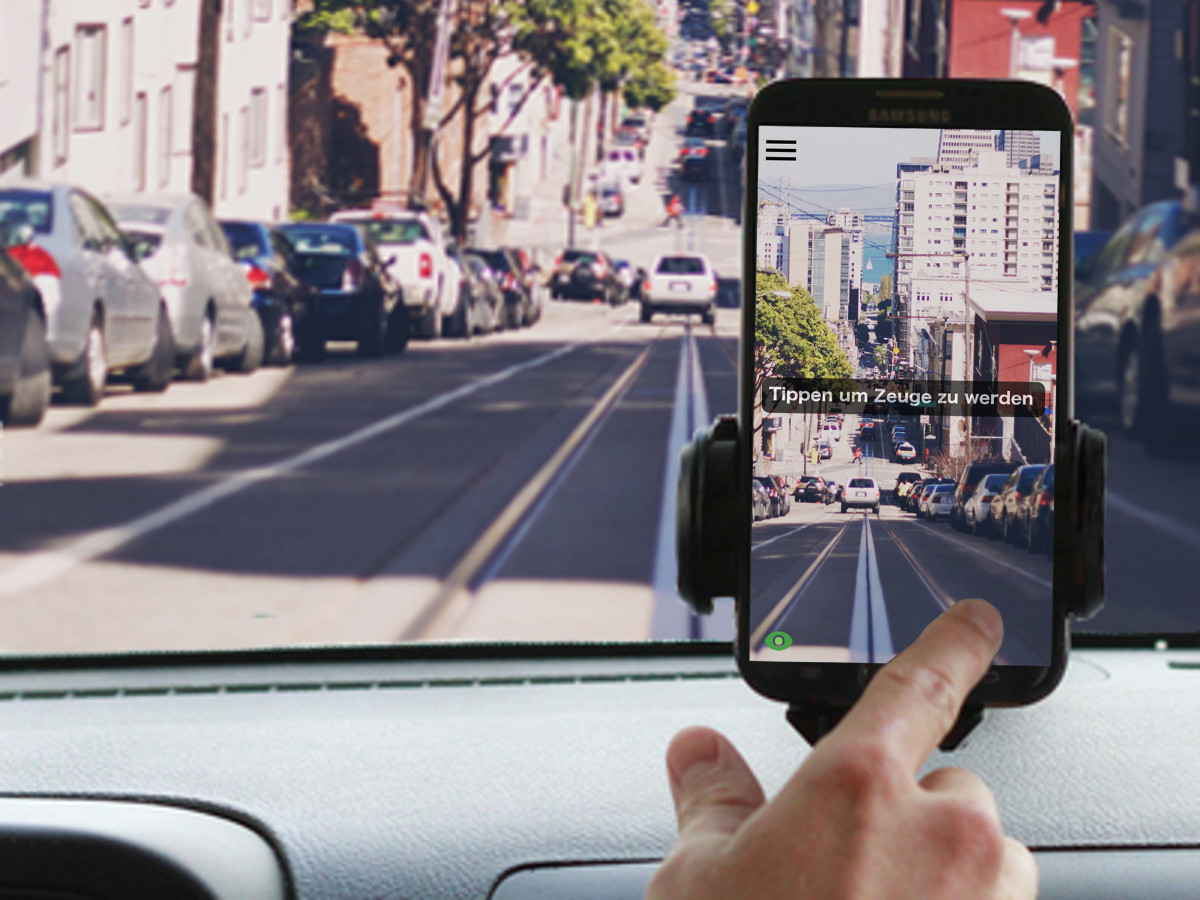
\includegraphics[width=\textwidth]{subtopicsFuncspec/Res//Mockups/Portrait_camera_view_car.jpg}\\[0.5cm]

Das Produkt ermöglicht es seinen Nutzern ihre Autofahrten zu überwachen, indem es durch die Handykamera den Straßenverkehr verfolgt und relevantes Videomaterial persistent abspeichert. Dieses wird bei Bedarf verwendet, um Unfallhergänge im Straßenverkehr zu dokumentieren. Dabei gilt es, dem deutschen Datenschutzrecht gerecht zu werden, indem Personen und personenbezogene Daten, wie zum Beispiel Autokennzeichen, unkenntlich gemacht werden. Die Anwendung bietet dem Nutzer dafür eine moderne und intuitive Bedienoberfläche.\newline
Zur Realisierung kann das Produkt in drei Hauptbestandteile aufgegliedert werden: Die Android App, den Web-Dienst und das Web-Interface. Diese Aufteilung wird in diesem Heft um Übersicht zu schaffen auch in nachfolgenden Kapiteln beibehalten.

\section{Musskriterien}
\subsection{App}
	\begin{enumerate}
	\renewcommand{\labelenumi}{\textbf{\theenumi}}
	\renewcommand{\theenumi}{PK\arabic{enumi}0}
	\setcounter{enumi}{99}
	\item Nutzer müssen sich einloggen um die App zu verwenden
	\item Nur registrierte Nutzer können die App verwenden
	\item Der Straßenverkehr wird durch die Handykamera beobachtet 
	\item Relevante Videodaten werden verschlüsselt abgespeichert
	\item Relevante Daten werden durch Auswertung der Sensordaten des Smartphones erkannt. Hierbei werden die Werte des G-Sensors ausgewertet
	\item Während der Aufnahme werden sämtliche Nutzereingaben und Sensordaten ignoriert
	\item Videodaten speichern relevante Metadaten
	\item Es wird ab dem Appstart mit dem Beobachten des Straßenverkehrs begonnen
	\item Es wird nur das Hochformat unterstützt
	\item Die Beobachtung läuft nur während sich die App im Vordergrund befindet
	\item Videodaten werden verschlüsselt, sobald sie persistiert werden
	\item Verschlüsselte Videodaten werden aufgelistet
	\item Verschlüsselte Videodaten können gelöscht werden
	\item Vom Nutzer ausgewählte verschlüsselte Videodaten werden an einen Webservice gesendet, der diese anonymisiert
	\item Geräte, auf denen Android API Level 19 (Android 4.4) und höhre läuft werden unterstützt
	\item Die Benutzeroberfläche wird für Geräte ab einer Displaydiagonale von 4 Zoll optimiert
	\item Wenn verschlüsselte Videodateien lange Zeit nicht zum anonymisieren ausgewählt wurden, wird der Nutzer benachrichtigt, dass er diese löschen kann
	\item Die aufnahmespezifischen Einstellungen werden angezeigt
	\item Die Standardsprache ist Deutsch
	\end{enumerate}
\subsection{Web-Dienst}
	\begin{enumerate}
	\renewcommand{\labelenumi}{\textbf{\theenumi}}
	\renewcommand{\theenumi}{PK\arabic{enumi}0}
	\setcounter{enumi}{199}
	\item Es existiert eine Schnittstelle, um Videodaten hochzuladen
	\item Von der App gesendete Videodaten werden anonymisiert
	\item Nach Abschluss der Anonymisierung wird der Nutzer per E-Mail benachrichtigt
	%\item Nach einer Registrierung bekommt der Nutzer eine Verifizierungs-E-Mail zugesendet
	\item Es existiert eine Schnittstelle, um Nutzeraccounts anzulegen
	\item Es existiert eine Schnittstelle, um Nutzeraccounts zu verwalten
	\item Es existiert eine Schnittstelle, um die Videodaten eines Nutzers verwalten zu können
	\item Nutzer müssen ihre E-Mail-Adresse verifizieren um sich einloggen zu können
	\item Die Kommunikation zwischen App und Webservice wird durch eine REST-API realisiert
	\item Die Kommunikation zwischen Web-Interface und Webservice wird durch eine REST-API realisiert
	\item Es existiert eine obere Schranke für die Anzahl der Videodateien, die ein Nutzer zur gleichen Zeit auf seinem Nutzeraccount online speichern kann
	\item Es wird Jetty verwendet
	\end{enumerate}
\subsection{Web-Interface}
	\begin{enumerate}
	\renewcommand{\labelenumi}{\textbf{\theenumi}}
	\renewcommand{\theenumi}{PK\arabic{enumi}0}
	\setcounter{enumi}{299}
	\item Es können Nutzeraccounts angelegt werden
	\item Es können Nutzeraccounts verwaltet werden
	\item Es können Videodaten verwaltet werden
	\item Es können Videodaten heruntergeladen werden
	\item Nur eingeloggte Nutzer haben Zugriff auf ihre Nutzerdaten
	\item Die Standardsprache ist Deutsch
	\end{enumerate}

\section{Wunschkriterien}
\subsection{App}
	\begin{enumerate}
	\renewcommand{\labelenumi}{\textbf{\theenumi}}
	\renewcommand{\theenumi}{WK\arabic{enumi}0}
	\setcounter{enumi}{99}
	\item Falls es Android zulässt wird die Beobachtung auch ausgeführt, wenn sich die App im Hintergrund befindet
	\item Sowohl Quer- als auch Hochformat werden unterstützt
	\item Die Beobachtung kann manuell gestartet und gestoppt werden
	\item Die Aufnahme kann manuell gestartet werden, auch wenn die Sensoren des Smartphones keinen Anlass dazu geben
	\item Es können Nutzeraccounts angelegt werden
	\item Es können Nutzeraccounts verwaltet werden
	\item Anonymisierte Videodateien können vom Server gelöscht werden
	\item Push-Benachrichtignungen vom Web-Service werden angezeigt
	\item Es können Hilfestellungen für die Bedienung der App angezeigt werden
	\item Anonymisierte Videodateien können heruntergeladen werden
	\item Anonymisierte Videodateien die zum Download bereit stehen und sich nicht auf dem Smartphone befinden werden aufgelistet
	\item Anonymisierte Videodateien die sich auf dem Smartphone befinden  werden aufgelistet
	\item Anonymisierte Videodateien können vom Speicher des Smartphones gelöscht werden
	\item Anonymisierte Videodateien die sich auf dem Smartphone befinden können angesehen werden
	\item Die aufnahmespezifischen Einstellungen können bearbeitet werden
	\item So lange die Sensoren des Smartphones anlass zur Aufnahme geben wird weiter aufgenommen
	\item Während der Aufnahme wird eine Möglichkeit angeboten die Aufnahme abzubrechen
	\end{enumerate}
\subsection{Web-Service}
	\begin{enumerate}
	\renewcommand{\labelenumi}{\textbf{\theenumi}}
	\renewcommand{\theenumi}{WK\arabic{enumi}0}
	\setcounter{enumi}{199}
	\item Die Zeit, die die Anonymisierung in Anspruch nehmen wird, wird geschätzt und and den Nutzer weitergeleitet
	\item Es wird eine Push-Benachrichtigung an das Smartphone gesendet, sobald die Anonymisierung der Videodaten abgeschlossen ist
	\item Videodaten werden maximal vier Wochen gespeichert
	\item Der Nutzer erhält eine Woche vor bevor ein Video glöscht wird eine E-Mail-Banchrichtigung
	\end{enumerate}
\subsection{Web-Interface}
	\begin{enumerate}
	\renewcommand{\labelenumi}{\textbf{\theenumi}}
	\renewcommand{\theenumi}{WK\arabic{enumi}0}
	\setcounter{enumi}{299}
	\item Das Produkt wird neuen Nutzern präsentiert
	\end{enumerate}

\section{Abgrenzungskriterien}
	\begin{enumerate}
	\renewcommand{\labelenumi}{\textbf{\theenumi}}
	\renewcommand{\theenumi}{AK\arabic{enumi}0}
	\item Das betrachten nicht anonymisierter Videodaten ist nicht möglich
	\item Videodaten werden nicht automatisch persistiert sobald die Beobachtung läuft
	\item Livestreams werden nicht unterstützt
	\item Die Anonymisierung findet nicht auf dem Smartphone statt
	\item Der Web-Service speichert Videodaten nicht auf unbegrenzte Zeit und in unbegrenzter Anzahl
	\item Vom Speicher des Smartphones werden Videodaten nicht automatisch gelöscht
	\item Von Nutzern zurückgelegte Wege und besuchte Orte werden nicht aufgezeichnet
	\item Die App ist nicht mit Windows Phone und iOS kompatibel
	\item Die App wird nicht für Tablets optimiert
	\end{enumerate}
\chapter{Produkteinsatz}

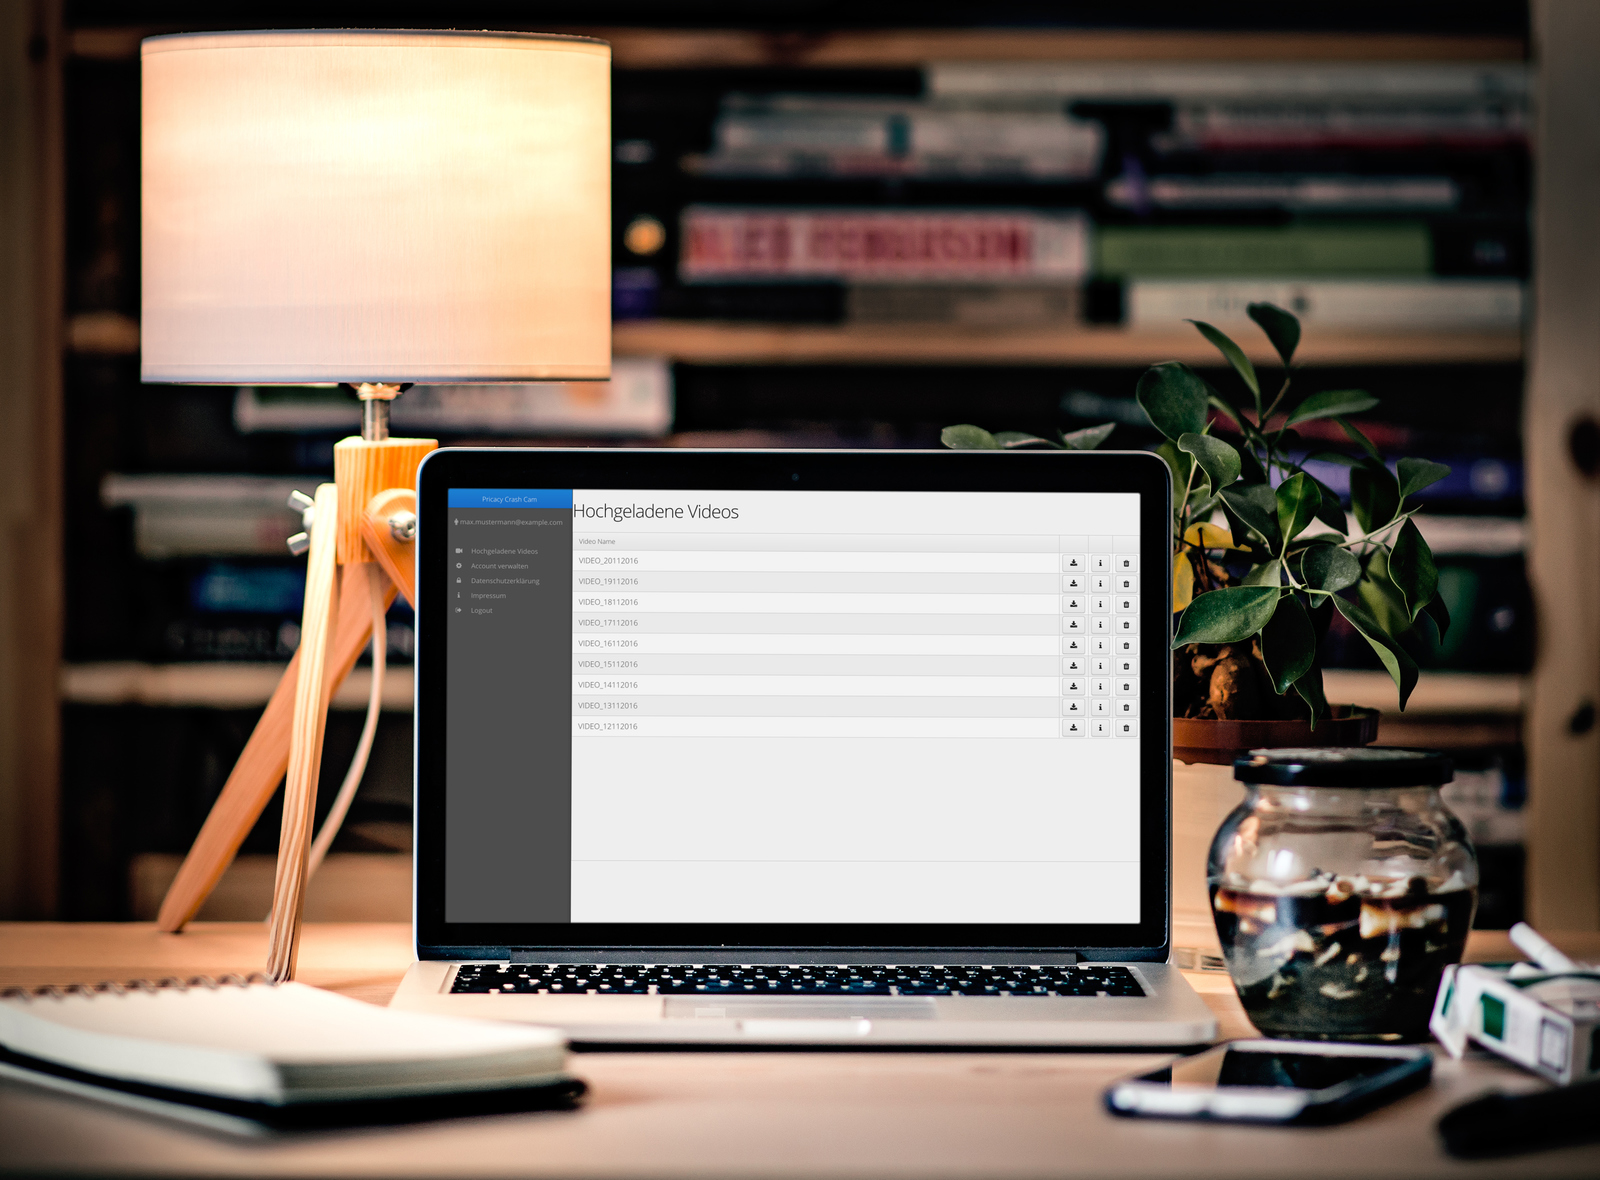
\includegraphics[width=\textwidth]{subtopicsFuncspec/Res/Mockups/Webinterface_desktop.jpg}

\section{Zielgruppe}
Die Privacy Dash Cam verfolgt zwei grundlegende Ziele: Eine Dash Cam für das \gls{Smartphone} anzubieten und ihren Einsatz mit dem deutschen Datenschutzrecht in Einklang zu bringen. Daraus lässt sich eine eindeutige Zielgruppe ableiten, die sich aus in Deutschland ud Österreich ansässigen Auto-, LKW und Motorrad-Fahrern zusammensetzt. Dabei haben sowohl Viel- als auch Gelegenheitsfahrer Bedarf an der Privacy Dash Cam. Darüber hinaus müssen Nutzer ein \gls{Smartphone} besitzen, welches den Geräteanforderungen der \gls{App} gerecht wird. Weiterhin werden Kenntnisse über die Benutzung des \glslink{Smartphone}{Smartphones}, Verständins der deutschen Sprache und ein Internetzugang für die Verwendung des Produktes vorrausgesetzt.

\section{Einsatz}
Nachdem die \gls{App} auf einem kompatiblen \gls{Smartphone} installiert und ein Nutzeraccount erstellt wurde, findet sie ihren Einsatz im Straßenverkehr. Der Nutzer platziert dazu sein \gls{Smartphone} mithilfe einer speziellen Halterung an der Frontscheibe seines Kraftfahrzeugs und ermöglicht so der Kamera ein deutliches Bild auf die Straße vor ihr. Darüber hinaus wird das \gls{Smartphone} nach dem Aufzeichnen von relevantem Videomaterial verwendet, um besagtes Material dem Webservice zum \gls{anonymisieren} zu senden.\newline
Das Web-Interface stellt die zweite Instanz dar, mit der der Nutzer direkt interagieren kann. Mit Hilfe dieser kann der Nutzer seinen Account verwalten und das vom \gls{Web-Dienst} \glslink{anonymisieren}{anonymisierte} Videomaterial herunterladen.


\chapter{Produktumgebung}

\section{Software}

\section{Hardware}

\section{Orgware (Netzwerkverbindung zum...)}

\section{Produktschnittstellen}
\chapter{Funktionale Anforderungen}

\section{\gls{App}}
\begin{enumerate}
\renewcommand{\labelenumi}{\textbf{\theenumi}}
\renewcommand{\theenumi}{FA\arabic{enumi}0}
\setcounter{enumi}{99}
\item \label{fa:anmeldeAnsicht} \textbf{Anzeigen der Anmeldeansicht} \hfill \\
Öffnet der Benutzer die \gls{App} und sind keine Nutzerdaten gespeichert~\eqref{fa:loginApp}, so gelangt er in die Anmeldeansicht, in der er sich anmelden kann. Das Erstellen von Benutzeraccounts ist hier \textbf{nicht} möglich.

\item \label{fa:Anmeldedaten}\textbf{Anmeldedaten speichern} \hfill \\
Anmeldedaten bestehen aus der E-Mail-Adresse und dem Passwort des Nutzers und werden lokal auf dem Gerät abgespeichert. Das Passwort wird als \gls{Hash-Code} gespeichert.

\item \label{fa:loginApp} \textbf{Anmelden in die \gls{App}} \hfill \\
Beim Appstart muss sich der Nutzer zunächst anmelden. Zum Anmelden müssen die Anmeldedaten~\eqref{fa:Anmeldedaten} des Nutzers korrekt in die entsprechenden Felder eingetragen sein. Nur verifizierte Nutzer~\eqref{fa:erstellAcc} können sich anmelden. Bei falschen Eingaben hat, erhält der Nutzer eine Fehlermeldung. Hat sich ein Nutzer bereits zuvor angemeldet, ohne sich wieder abzumelden, gelangt der Nutzer direkt zur Kamera-Ansicht. Die Überprüfung der gespeicherten Anmeldedaten erfolgt dann erst beim Hochladen von Videodaten auf den Server~\eqref{fa:vidHochladen}.

\item \label{fa:logOut}\textbf{Abmelden von einem Benutzeraccount} \hfill \\
Klickt ein Benutzer im Menü auf ``abmelden'', so wird er auf die Anmeldeansicht~\eqref{fa:anmeldeAnsicht} geleitet und seine lokalen Anmeldedaten~\eqref{fa:Anmeldedaten} vom Gerät gelöscht.

\item \label{fa:Beobachtungsmodus}\textbf{Ausführen des Beobachtungsmodus} \hfill \\
Die Kamera kann sich bei aktiver Kamera in zwei Modi befinden: Im Beobachtungsmodus oder im Aufnahmemodus~\eqref{fa:Aufnahmemodus}.
Im Beobachtungsmodus werden Kamerabilder nicht ~\eqref{fa:Persistieren} sondern nur der \gls{Ringpuffer}~\eqref{fa:Ringpuffer} beschrieben. Die \gls{G-Sensor}-Daten werden ausgewertet und es wird auf einen charakteristischen Ausschlag des G-Sensors ~\eqref{fa:automUebergang}, oder manuelles Auslösen ~\eqref{fa:manUebergang} gewartet.

\item \label{fa:Statussymbol}\textbf{Anzeigen des Statussymbols} \hfill \\
Der aktuelle Kameramodus wird dem Nutzer durch ein blinkendes Statussymbol am Bildschirmrand visualisiert. Im Beobachtungsmodus hat es eine grüne Farbe, im Aufnahmemodus hat es eine rote Farbe.

\item \textbf{Stoppen der Beobachtung} \hfill \\
Wenn der Benutzer die Kamera-Ansicht ~\eqref{fa:kamAnsicht} während der Beobachtung verlässt, oder die \gls{App} schließt, wird die Beobachtung automatisch beendet.

\item \label{fa:automUebergang}\textbf{Durch \gls{G-Sensor} ausgelöster Übergang in den Aufnahmemodus} \hfill \\
Werden die in~\eqref{na:GSensfront} -~\eqref{na:GSensvert} definierten Richtwerte des G-Sensors überschritten, während die \gls{App} die Kamera-Ansicht~\eqref{fa:kamAnsicht} anzeigt, geht die Kamera in den Aufnahmemodus über~\eqref{fa:Aufnahmemodus}. 

\item \label{fa:manUebergang}\textbf{Manueller Übergang in den Aufnahmemodus} \hfill \\
Befindet sich die Kamera im Beobachtungsmodus~\eqref{fa:Beobachtungsmodus}, geht sie nach doppeltem Tippen auf die Vorschaufläche der Kamera-Ansicht~\eqref{fa:kamAnsicht} in den Aufnahmemodus ~\eqref{fa:Aufnahmemodus} über.

\item \label{fa:Aufnahmemodus}\textbf{Ausführen des Aufnahmemodus} \hfill \\
Im Aufnahmemodus wird der \gls{Ringpuffer} zunächst für 30 Sekunden beschrieben ~\eqref{fa:Ringpuffer}und anschließend der komplette Inhalt des Puffers im Hintergrund persistiert~\eqref{fa:Persistieren}. Weitere \gls{G-Sensor}-Ausschläge, sowie Nutzereingaben werden während sich die Kamera im Aufnahmemodus befindet ignoriert. Die Messwerte des G-Sensors, Zeit und Auslöseart (\eqref{fa:automUebergang}, ~\eqref{fa:manUebergang}) werden in die \gls{Metadaten} der Videodatei geschrieben. Nach Ablauf der erwähnten 30 Sekunden wechselt die Kamera wieder zurück in den Beobachtungsmodus~\eqref{fa:Beobachtungsmodus}.

\item \label{fa:Ringpuffer}\textbf{\gls{Ringpuffer} beschreiben} \hfill \\
Im Beobachtungsmodus ~\eqref{fa:Beobachtungsmodus} wird der \gls{Ringpuffer} mit den Videodaten der Kamera beschrieben. Die Tonspur wird verworfen. Die auf dem Ringpuffer vorhanden Daten sind nicht verschlüsselt und daher dem Benutzer auch nicht zugänglich. Der Ringpuffer hält bis zu 1 Minute Videomaterial ~\eqref{na:Ringpuffer}.

\item \label{fa:Persistieren}\textbf{Video \gls{persistieren}} \hfill \\
Beim Persistieren, werden die Videodaten zunächst verschlüsselt~\eqref{fa:Verschluesselung} und daraufhin auf dem internen Speicher hinterlegt.

\item \label{fa:Verschluesselung}\textbf{Verschlüsseln eines Videos} \hfill \\
Dem Nutzer zugängliche Videodaten werden durch das unter~\ref{sec:Verschlüsselung} beschriebene hybride Verschlüsselungsverfahren verschlüsselt.

\item \begin{minipage}[t]{\linewidth} 
\textbf{Anzeigen des Menüs} \hfill \\
	\begin{wrapfigure}{r}{0.4\linewidth}
		\vspace{-70pt}
  		\begin{center}
   			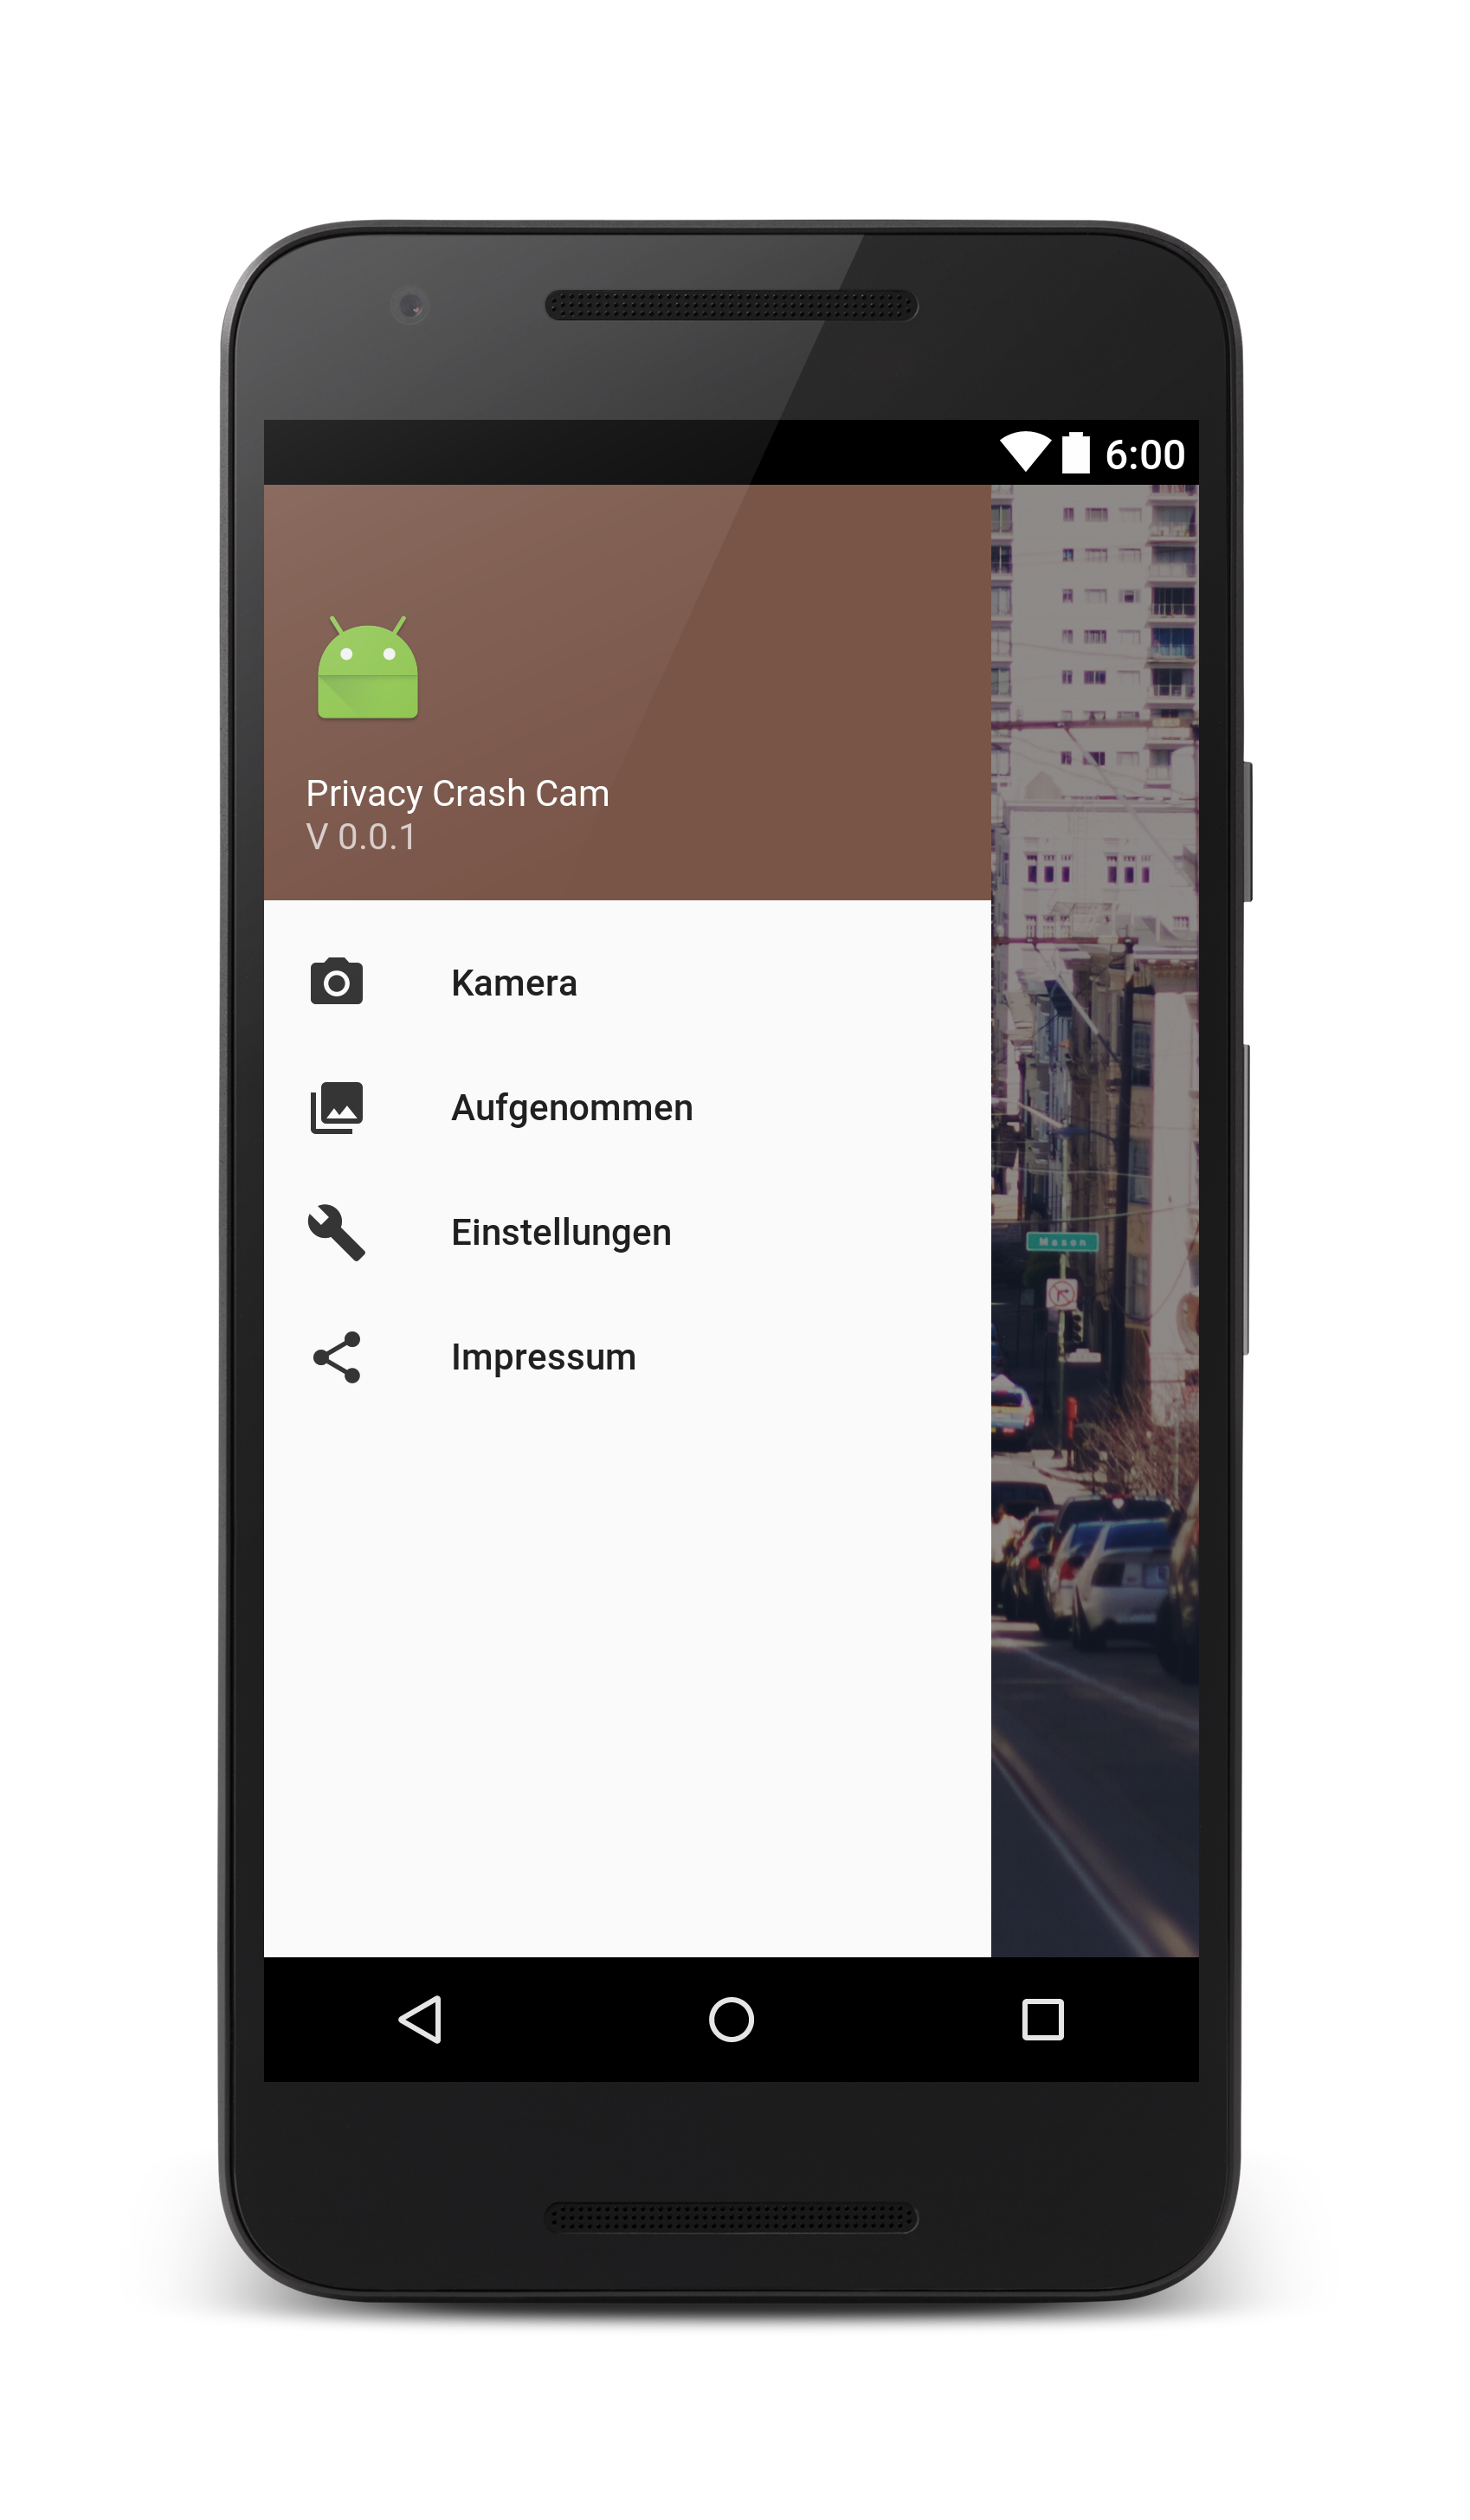
\includegraphics[width=0.4\textwidth]{subtopicsFuncspec/Res/Mockups/Portrait_camera_view_menu_phone.png}
  		\end{center}
  		\vspace{-20pt}
  		\vspace{-10pt}
	\end{wrapfigure}
Drückt der Benutzer den ``Menü-Button'' in der oberen linken Ecke des Bildschirms, so öffnet sich das Menü. Wenn sich die Kamera im Beobachtungsmodus befindet, während das Menü geöffnet wird, wird die Aufnahme nicht gestoppt. In dem Menü hat der Benutzer die Möglichkeit zwischen den verschiedenen \gls{App}-Ansichten Kamera-Ansicht~\eqref{fa:kamAnsicht}, Liste der persistierten Videos~\eqref{fa:vidAnsicht}, Einstellungs-Ansicht~\eqref{fa:einstAnsicht} und Impressum-Ansicht~\eqref{fa:imprAnsicht} zu wählen, oder sich abzumelden~\eqref{fa:logOut}.

\item \label{fa:kamAnsicht}\textbf{Anzeigen der Kamera-Ansicht} \hfill \\
Wenn sich ein Benutzer gerade angemeldet hat oder im Menü die Option ``Kamera'' wählt, so gelangt er zu der Kamera-Ansicht. Dort sieht er die Vorschau seines Kamerabildes. Zudem gelangt der automatisch in den Beobachtungsmodus~\eqref{fa:Beobachtungsmodus}.

\item \label{fa:vidAnsicht}\textbf{Anzeigen der Liste der \glslink{persistieren}{persistierten} Videos} \hfill \\
Wählt der Benutzer im Menü die Option ``Aufgenommen'', so gelangt er zu einer Ansicht, in dem ihm seine persistierten~\eqref{fa:Persistieren} Videos chronologisch aufgelistet werden. Der Nutzer kann dort Videos hochladen~\eqref{fa:vidHochladen}, löschen~\eqref{fa:vidLöschen}, oder Videoinformationen einsehen~\eqref{fa:metaVerschlVid}.
\end{minipage}

\item \label{fa:vidHochladen}\textbf{Hochladen von gespeicherten Videos} \hfill \\
Wenn der Nutzer auf den ``Upload-Button'' klickt,so wird ein Bestätigungsdialog geöffnet. Falls der Benutzer bestätigt, schickt die \gls{App} eine Anfrage an den Server~\eqref{fa:vidHochladen} das Video hochzuladen. Bricht der Benutzer den Dialog ab, bleibt er in der Listenansicht seiner Videos. Falls beim Hochladen ein Fehler auftritt, wird eine Fehlermeldung der App bzw. die vom Server gesendete Fehlermeldung angezeigt.

\item \label{fa:vidLöschenApp}\textbf{Löschen von gespeicherten Videos} \hfill \\
Klickt der Benutzer auf das ``Löschen-Symbol'', so wird ein Bestätigungsdialog geöffnet. Falls der Benutzer bestätigt, wird das Video aus der Liste seiner persistierten ~\eqref{fa:Persistieren} Videos entfernt und vom Gerät gelöscht. Bricht der Benutzer den Dialog ab, bleibt er in der Listenansicht seiner Videos.

\item \label{fa:vidLöschenDialog}\textbf{Anzeigen einer Benachrichtigung zum Löschen von Videos} \hfill \\
Beim Anmelden und bei jedem Appstart wird geprüft, ob persistierte ~\eqref{fa:Persistieren} Videos bereits seit über 4 Wochen auf seinem Gerät gespeichert sind. Ist dies so wird ihm ein Dialog angezeigt, der ihn auf diesen Umstand hinweist. Dort wird ihm angeboten, das Video zu löschen~\eqref{fa:vidLöschenApp}. Bricht er den Dialog ab, gelangt er wie üblich in die Kamera-Ansicht~\eqref{fa:kamAnsicht}.

\item \label{fa:metaVerschlVid}
\textbf{Einsehen von Video-Daten der verschlüsselten Videos} \hfill \\
\begin{minipage}[t]{\linewidth}
	\begin{wrapfigure}{r}{0.4\linewidth}
		\vspace{-35pt}
  		\begin{center}
   			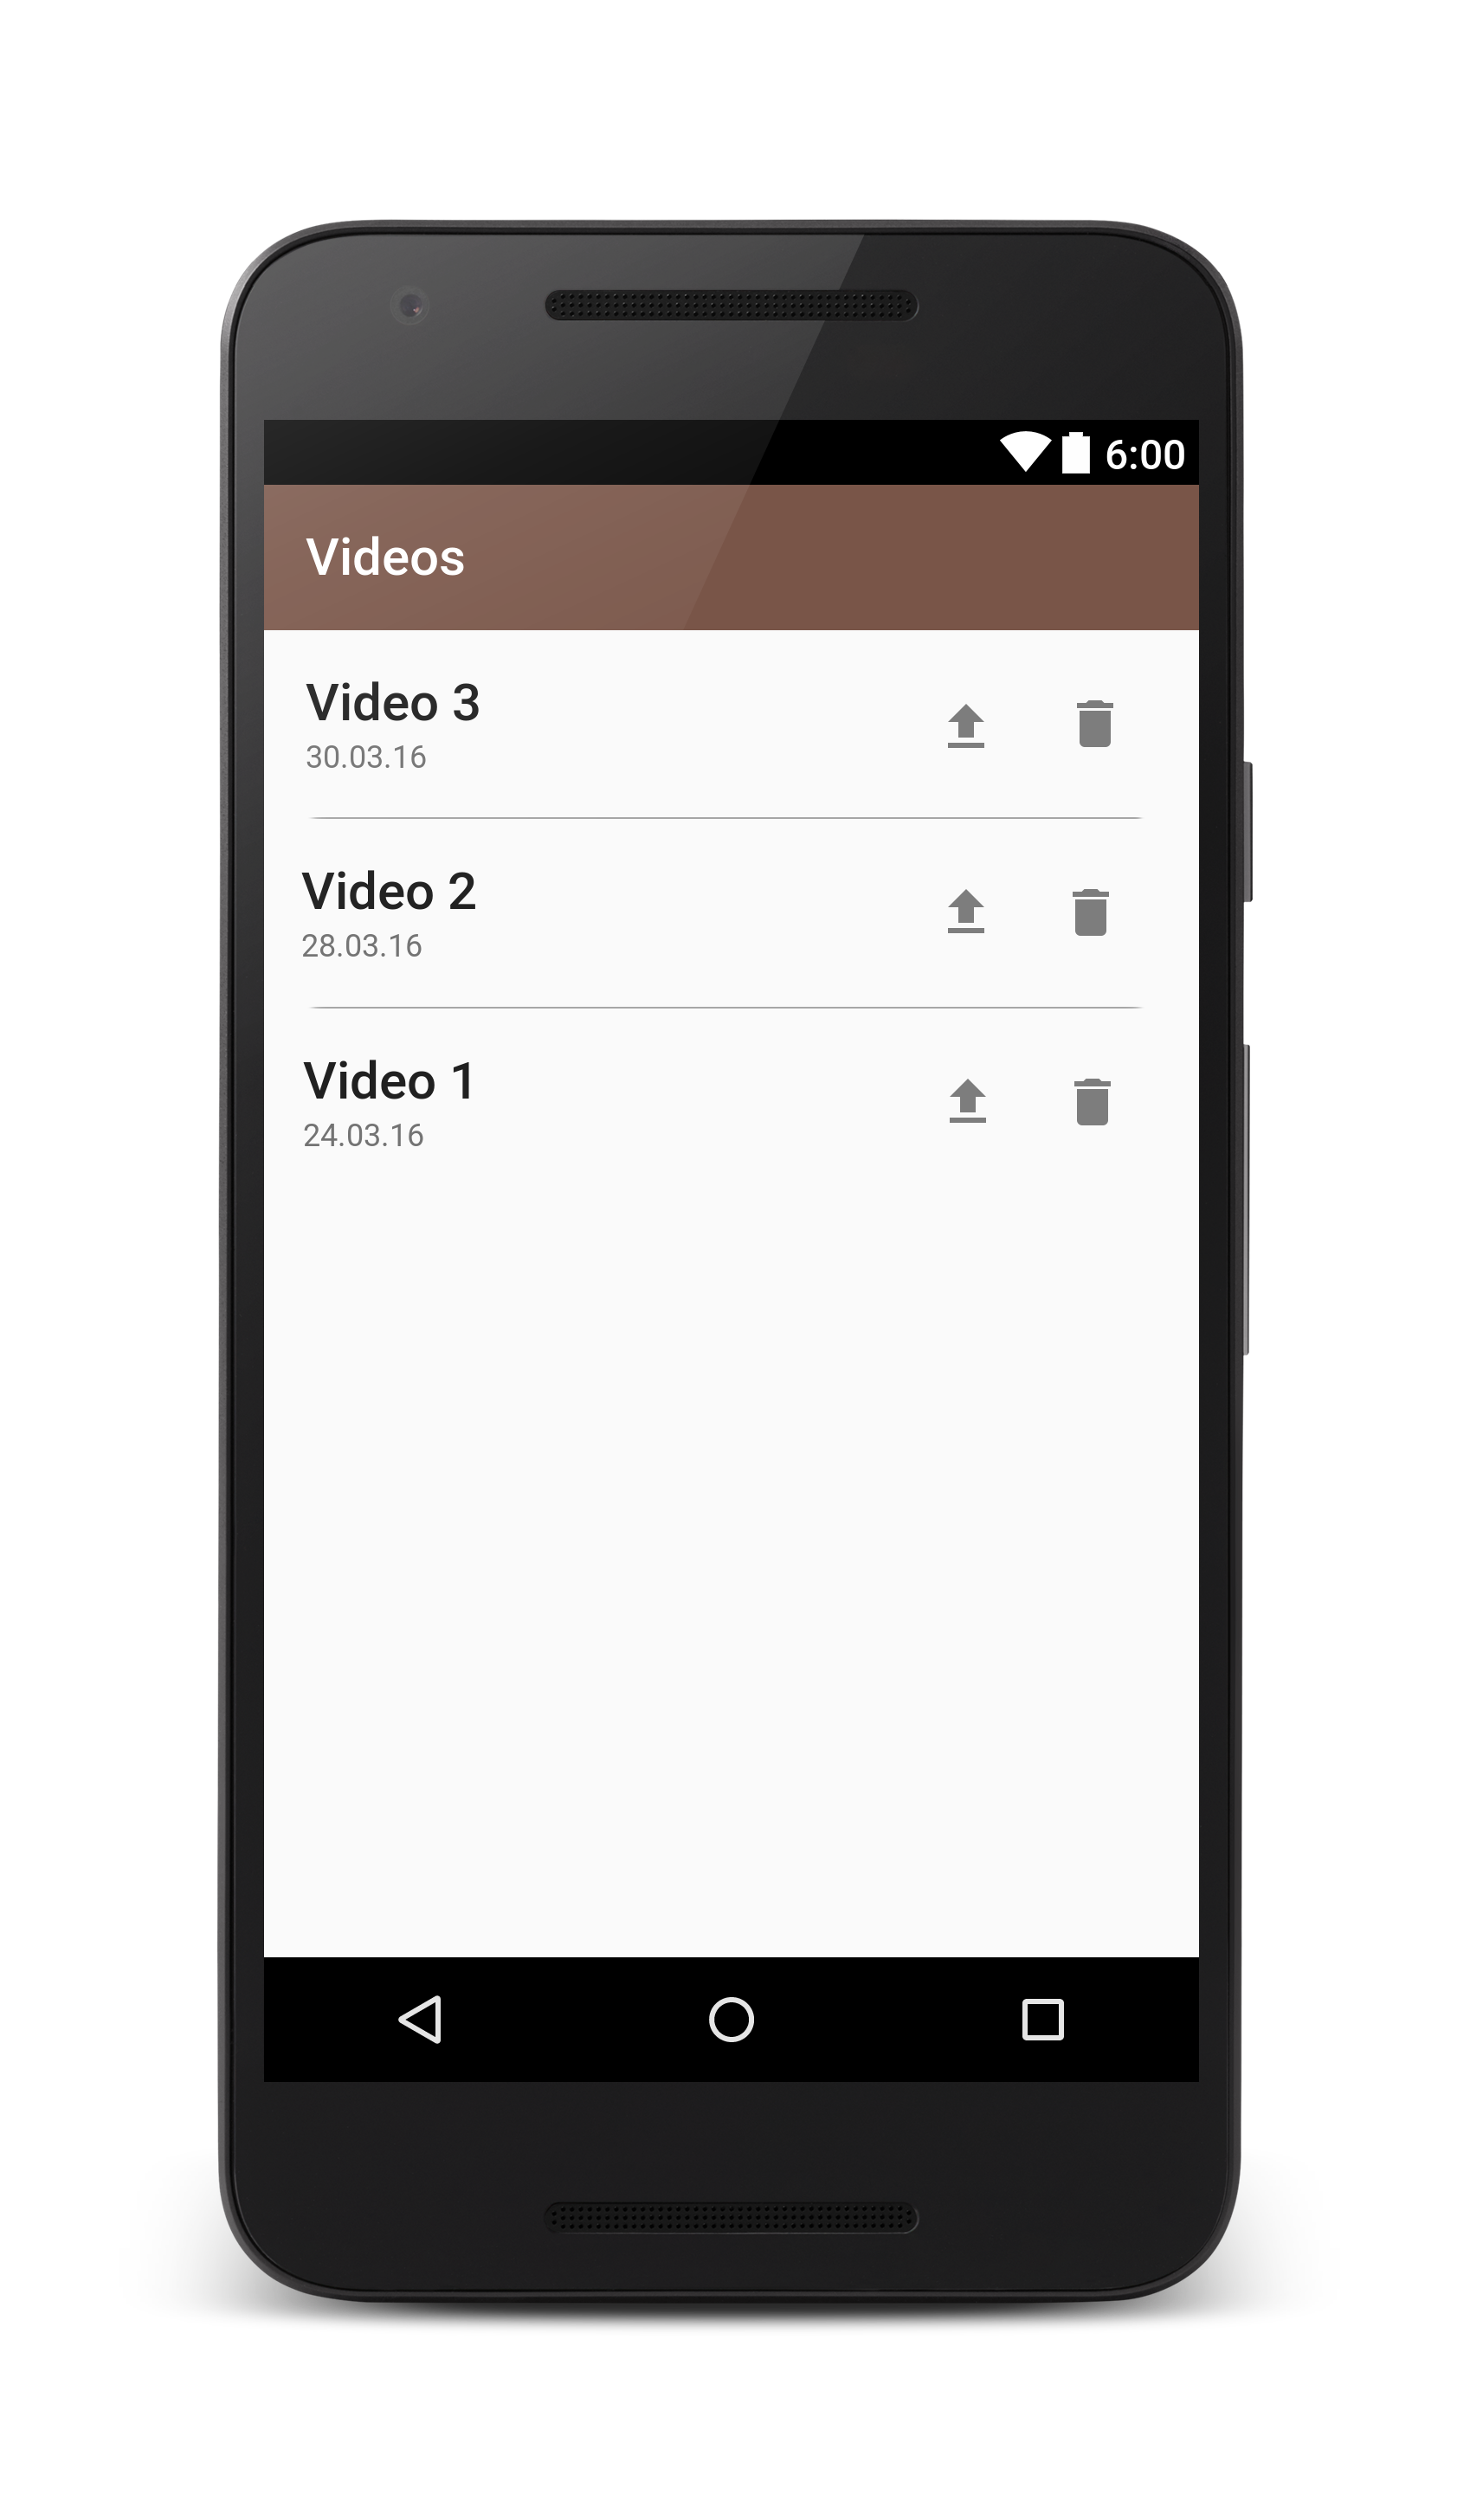
\includegraphics[width=0.4\textwidth]{subtopicsFuncspec/Res/Mockups/Videos_list1_phone.png}
  		\end{center}
  		\vspace{-20pt}
  		\vspace{-10pt}
	\end{wrapfigure}
Klickt der Benutzer lange auf ein Video, wird ein Fenster geöffnet, das dem Benutzer die Video-\gls{Metadaten} (Erstellungsdatum, Größe, Auflösung, Dauer, Auslöseart, \gls{G-Sensor}-Daten) als Dialog anzeigt. Schließt der Nutzer den Dialog, kehrt er zu der Liste seiner Videos~\eqref{fa:vidAnsicht} zurück.

\item \label{fa:einstAnsicht}\textbf{Anzeigen der Einstellungen} \hfill \\
Wählt der Benutzer im Menü die Option ``Einstellungen'', so werden dem Nutzer die Einstellungen angezeigt (Auflösung, Bildwiederholrate, Größe \gls{Ringpuffer}) angezeigt. Diese sind mit Standardparametern festgelegt.

\item \label{fa:imprAnsicht}\textbf{Anzeigen rechtlicher Informationen} \hfill \\
Wählt der Benutzer im Menü die Option ``Impressum'', gelangt er zur Impressums-Ansicht. Von dort kann er sich das Impressum~\eqref{fa:imprAnzeigen} und die Datenschutzerklärung~\eqref{fa:datenschAnzeigen} anzeigen lassen.
\end{minipage}

\item \label{fa:imprAnzeigen}\textbf{Anzeigen des Impressums} \hfill \\
Wählt der Benutzer ``Impressum'' auf der Impressum-Ansicht, wird ein Dialog angezeigt, der das Impressum anzeigt.

\item \label{fa:datenschAnzeigen}\textbf{Anzeigen der Datenschutzerklärung} \hfill \\
Wählt der Benutzer ``Datenschutzerklärung'' auf der Impressum-Ansicht, wird ein Dialog angezeigt, der die Datenschutzerklärung anzeigt.

\end{enumerate}




\section{\gls{Web-Dienst}}
\begin{enumerate}
\renewcommand{\labelenumi}{\textbf{\theenumi}}
\renewcommand{\theenumi}{FA\arabic{enumi}0}
\setcounter{enumi}{199}

\item \label{fa:empfangVid} \textbf{Empfangen eines Videos von der \gls{App}} \hfill \\
Bekommt der \gls{Web-Dienst} eine Anfrage von der App, ein Video hochzuladen, so überprüft er zunächst, ob er die Anfrage bearbeiten kann, oder ob bereits zu viele andere Anfragen gestellt wurden~\eqref{na:paralleleZugriffe}. Ist dies nicht der Fall, so entschlüsselt er das Video~\eqref{fa:entschVideo} und beginnt die Anonymisierung~\eqref{fa:anonymVideo}. Bei Fehlern bei der Anfrage bzw. wenn der Server die Anfrage annimmt, beantwortet der Server die Anfrage mit einer Fehlermeldung bzw. Erfolgsmeldung.

\item  \label{fa:entschVideo}\textbf{Entschlüsseln eines empfangenen Videos} \hfill \\
Bevor der \gls{Web-Dienst} die Bearbeitung des Videos beginnt, entschlüsselt er das empfangene verschlüsselte Video ~\ref{sec:Verschlüsselung}. Das entschlüsselte Video wird lokal temporär gespeichert.

\item  \label{fa:anonymVideo}\textbf{\glslink{anonymisieren}{Anonymisierung} des Videos} \hfill \\
Der \gls{Web-Dienst} analysiert zunächst das Video~\eqref{fa:relBildbereiche}. Die dadurch gefundenen, für die Anonymisierung relevanten Bildbereiche werden mithilfe von Bildfiltern unkenntlich gemacht.

\item  \label{fa:relBildbereiche}\textbf{Identifizieren der relevanten Bildbereiche} \hfill \\
Der \gls{Web-Dienst} nimmt das entschlüsselte Video und lässt einen Bildfilter über das Video laufen, der die für die Anonymisierung relevanten Bildbereiche (Gesichter, Nummernschilder, etc.) erkennt.

\item \label{fa:speichVideo}\textbf{Abspeichern eines \glslink{anonymisieren}{anonymisierten} Videos} \hfill \\
Nachdem das Video anonymisiert wurde, wird es auf dem Server gespeichert und alle temporären Dateien gelöscht. Das gespeicherte Video wird der Videoverwaltung hinzugefügt, damit es vom Benutzer eingesehen und bearbeitet werden kann. Wenn ein Benutzer die maximale Anzahl Videos pro Account~\eqref{na:VideoKap} überschreitet, wird automatisch das älteste Video des Accounts auf dem Server gelöscht.

\item \label{fa:accSpeichern}\textbf{Speichern eines Accounts} \hfill \\
Wenn ein Nutzer sich registriert~\eqref{fa:erstellAcc}, werden seine Accountdaten auf dem Server gespeichert. Passwörter werden ausschließlich als \gls{Hash-Code} abgelegt. Zusätzlich wird hinterlegt, dass der Account noch nicht verifiziert wurde.

\item \label{fa:vidHerunterladen}\textbf{Video herunterladen} \hfill \\
Möchte ein Nutzer ein anonymisiertes Video herunterladen~\eqref{fa:anonymVidherunt}, so stellt der Server die Videodaten bereit und startet das Herunterladen.

\item \label{fa:vidLöschen}\textbf{Video löschen} \hfill \\
Möchte ein Nutzer eins seiner hochgeladenen Videos löschen~\eqref{fa:anonymVidlösch}, so werden die Videodaten vom Server gelöscht.

\item \label{fa:mailSenden}\textbf{Versenden einer Bestätigungsmail} \hfill \\
Hat ein Benutzer das Anmeldeformular~\eqref{fa:erstellAcc} ausgefüllt, so versendet der \gls{Web-Dienst} eine Bestätigungsmail. Klickt der Benutzer auf den dort vorhanden Bestätigungslink so wird der Account verifiziert.

\item \label{fa:accLöschen}\textbf{Löschen eines Accounts} \hfill \\
Wenn der Nutzer seinen Account löschen will werden zunächst alle, von ihm hochgeladenen Videos vom Server gelöscht. Wird gerade ein Video des Benutzers anonymisiert, so wird dieses nach der Anonymisierung nicht gespeichert. Danach werden die Accountdaten des Nutzers gelöscht.

\item \label{fa:accÄndern}\textbf{Accountdaten ändern} \hfill \\
Hat der Nutzer seine Accountdaten geändert~\eqref{fa:accDatBearb}, so werden die Änderungen entsprechend auf dem Server hinterlegt.

\end{enumerate}





\section{\gls{Web-Interface}}
\begin{enumerate}
\renewcommand{\labelenumi}{\textbf{\theenumi}}
\renewcommand{\theenumi}{FA\arabic{enumi}0}
\setcounter{enumi}{299}
\item \label{fa:loginWeb} \textbf{Anzeigen der Anmeldeansicht} \hfill \\
Ruft der Nutzer die Privacy-Crash-Cam-Webseite auf, so gelangt er zu der Anmeldeansicht. Dort kann sich der Benutzer anmelden~\eqref{fa:weblogIn} oder sich registrieren~\eqref{fa:erstellAcc}.

\item \label{fa:erstellAcc}\textbf{Erstellen eines Benutzeraccount} \hfill \\
Klickt der Benutzer auf "'Account erstellen"' so öffnet sich der Registrierungsdialog. Dort wird der Nutzer gebeten eine \gls{E-Mail} Adresse angegeben. Zudem muss er ein Passwort auswählen und bestätigen. Klickt der Nutzer auf "'Registrierung abschließen"' werden die Eingaben überprüft. Schlägt dies fehl bleibt der Benutzer in dem Registrierungsdialog. Nach dem Erstellen eines Benutzeraccounts~\eqref{fa:accSpeichern} sendet der Server eine Bestätigungsmail~\eqref{fa:mailSenden}.

\item \label{fa:weblogIn}\textbf{Anmelden auf der Webseite} \hfill \\
Zum Anmelden auf die Webseite müssen Benutzername und Passwort korrekt in die entsprechenden Felder eingetragen sein. Nur verifizierte Nutzer~\eqref{fa:mailSenden} können sich anmelden. Bei falschen Eingaben kehrt er zur Anmeldeansicht zurück und erhält eine Fehlermeldung.

\item \textbf{Anzeigen der Menüleiste} \hfill \\
Befindet sich der Nutzer in einer anderen Ansicht als der Anmeldeansicht, so befindet sich am linken Rand der Websteite die Menüleiste. Dort kann der Nutzer die Liste der \glslink{anonymisieren}{anonymisierten} Videos~\eqref{fa:anonymVidAnzeigen}, seinen Account bearbeiten~\eqref{fa:accBearb}, die Datenschutzerklärung einsehen~\eqref{fa:datenschutzWeb}, das Impressum einsehen~\eqref{fa:impressumWeb}, oder sich abmelden~\eqref{fa:weblogOut}.

\item \label{fa:anonymVidAnzeigen}\textbf{Anzeigen der Liste der \glslink{anonymisieren}{anonymisierten} Videos} \hfill \\
Hat sich ein Benutzer eingeloggt, wird er automatisch auf diese Ansicht weitergeleitet. Hier werden die, von dem Nutzer hochgeladenen Videos chronologisch aufgelistet. Der Nutzer kann Videos herunterladen~\eqref{fa:anonymVidherunt}, löschen~\eqref{fa:anonymVidlösch}, ein Preview einsehen~\eqref{fa:anonymVidprev}, oder die Videoinformationen einsehen~\eqref{fa:anonymViddaten}.

\item \label{fa:anonymVidherunt}\textbf{Herunterladen von \glslink{anonymisieren}{anonymisierten} Videos} \hfill \\
Durch einen Klick auf das ``Herunterlade-Icon'' wird ein Speicherdialog geöffnet. Nachdem der Nutzer einen Speicherort ausgewählt hat, wird das Video heruntergeladen~\eqref{fa:vidHerunterladen}. Bricht der Benutzer den Dialog ab, bleibt er in der Listenansicht seiner Videos.

\item \label{fa:anonymVidlösch}\textbf{Löschen eines \glslink{anonymisieren}{anonymisierten} Videos} \hfill \\
Durch den Klick auf das ``Löschen-Symbol'' wird ein Bestätigungsdialog geöffnet. Falls der Benutzer bestätigt, wird das Video aus der Liste seiner hochgeladenen Videos entfernt und vom Server gelöscht~\eqref{fa:vidLöschen}. Bricht der Benutzer den Dialog ab, bleibt er in der Listenansicht seiner Videos.

\item \label{fa:anonymViddaten}\textbf{Einsehen von Video-Daten der \glslink{anonymisieren}{anonymisierten} Videos} \hfill \\
Klickt der Benutzer auf das ``Info-Symbol'', so wird ein Fenster geöffnet, das dem Benutzer die Video-\gls{Metadaten} (Erstellungsdatum, Datum der Anonymisierung, Größe, Auflösung, Dauer) anzeigt.

\item \label{fa:accBearb}\textbf{Bearbeiten eines Benutzeraccounts} \hfill \\
Klickt ein Benutzer in der Menüleiste auf ``Account bearbeiten'', so wird ein Fenster geöffnet in, dem der Nutzer auswählen kann ob er seine Accountdaten ändern, oder seinen Account löschen will.

\item \label{fa:accLöschenWeb}\textbf{Account Löschen} \hfill \\
Klickt der Benutzer in dem Fenster~\eqref{fa:accBearb} auf ``Account Löschen'', so öffnet sich ein Bestätigungsdialog, in dem der Benutzer gefragt wird, ob er wirklich seinen Account löschen will. Bestätigt dieser, so gelangt er zu der Anmeldeansicht~\eqref{fa:loginWeb} und sein Account wird gelöscht~\eqref{fa:accLöschen}.

\item \label{fa:accDatBearb}\textbf{Accountdaten bearbeiten} \hfill \\
Klickt der Benutzer in dem Fenster~\eqref{fa:accBearb} auf ``Accountdaten ändern'', so kann er sein Passwort ändern. Dies macht er, in dem er zunächst in ein Feld sein altes Passwort und danach in zwei Felder sein neues gewünschtes Passwort eingibt. Stimmt das alte Passwort und stimmen die zwei Felder für das neue Passwort überein, so werden die Daten auf dem Server entsprechend geändert~\eqref{fa:accÄndern}.

\item \label{fa:impressumWeb} \textbf{Anzeigen des Impressums} \hfill \\
Klickt der Benutzer in der Menüleiste auf ``Impressum'', so wird eine Sicht geöffnet, in der der Nutzer das Impressum einsehen kann.

\item \label{fa:datenschutzWeb} \textbf{Anzeigen der Datenschutzerklärung} \hfill \\
Klickt der Benutzer in der Menüleiste auf ``Datenschutz'', so wird eine Sicht geöffnet, in der der Nutzer die Datenschutzerklärung und die AGB einsehen kann.

\item \label{fa:weblogOut}\textbf{Anmelden von der Webseite} \hfill \\
Klickt ein Benutzer in der Menüleiste auf ``Abmelden'', so wird er auf die Anmeldeansicht~\eqref{fa:loginWeb} zurückgeleitet. Schließt ein Nutzer die Webseite, so wird er automatisch ausgeloggt.

\end{enumerate}
\chapter{Produktdaten}

\section{App-Daten}
\begin{description}
\item[PD Kundendaten]\hfill \\
Es werden Nachname, Vorname sowie die E-Mail Adresse des Kunden gespeichert.
\item[PD Einstellungen]\hfill \\
Es werden Einstellungen der Kamera, sprich die Auflösung der Aufnahme.
\item[PD Ringpuffer]\hfill \\
Es werden eine Minute an Video Material im Ringpuffer gespeichert.
\item[PD Videodaten]\hfill \\
Es werden Videodaten, sowie Ort und Zeit in die Meta-Daten des Videos gespeichert.
\end{description}

section{Web-Service}
\begin{description}
\item[PD Videodaten]\hfill \\
Es werden Temporär Videodaten, sowie Ort und Zeit in den Meta-Daten des Videos gespeichert.
\end{description}

\section{Webinterface Daten}
\begin{description}
\item[PD Kundendaten]\hfill \\
Es werden Nachname, Vorname sowie die E-Mail Adresse des Kunden gespeichert. Jeder Kunde bekommt eine einzigartige ID zugewiesen.
\item[PD Videodaten]\hfill \\
Es werden anonymisierte Videodaten, sowie Ort und Zeit aus des Meta-Daten des Videos gespeichert. Das Tonsignal wird nicht gespeichert.
\end{description}



\section{Nichtfunktionale Anforderungen}
\chapter{Globale Testf\"alle}
\section{Erkl\"arung zur Qualit\"atssicherung}
Wir teilen die Testphase in mehrere Teilphasen ein, um sowohl Komponenten für sich, als auch ihr Zusammenarbeiten separat zu testen. Automatisierte Tests werden das Backend und Frontend testen. Zudem werden manuelle Tests zur \"Uberpr\"ufung der Bedienbarkeit durchgef\"uhrt.  Das Ziel ist, 80 Prozent des geschriebenen Codes ausf\"uhrlich zu testen.

\subsection{Komponenten-Tests}
In den Komponenten-Tests werden wir unsere drei Komponenten, die \gls{App}, das \gls{Web-Interface} und den \gls{Web-Dienst}, unabhängig voneinander testen.

\subsection{Integration-Tests}
In den Integration-Tests wird die Kommunikation zwischen den Komponenten getestet. In dieser Phase wird die korrekte Implementierung und Funktion der Schnittstellen sichergestellt.

\subsection{System-Tests}
Die Software wird in einer realen Umgebung installiert und dort unter realen Bedingungen von uns getestet.

\section{Testszenarien}
\subsection{Komponenten-Tests}

\subsubsection{\gls{App}}
\begin{enumerate}[\bfseries{TK}10]  
\setcounter{enumi}{99}{}

\item \textbf{Erstmaliges Starten der \gls{App}} \hfill\\  
Beim ersten Start der App wird die Anmeldeansicht angezeigt.

\item \textbf{Accountanmeldung} \hfill\\  
In der Anmeldeansicht wird der Benutzer aufgefordert, sich anzumelden. Nach erfolgreicher Anmeldung geht die \gls{App} in den Beobachtungsmodus \"uber.

\item \textbf{Men\"u \"offnen} \hfill\\
Die \gls{App} befindet sich im Beobachtungsmodus. Nach Klicken des Men\"ubuttons wird das Men\"u angezeigt.

\item \textbf{Accountabmeldung} \hfill\\  
Die App zeigt das Men\"u. Klickt der Benutzer auf ``abmelden'', werden die Benutzerdaten von der App gelöscht und er gelangt zur Anmeldeansicht.

\item \textbf{Starten der \gls{App} nach Erstanmeldung} \hfill\\  
Bei Start der App wird die Kameraansicht gezeigt, und die App befindet sich im Beobachtungsmodus. %KOMMA MUSS DA SEIN!!!

\item \textbf{Beobachtungsmodus} \hfill\\
Im Beobachtungsmodus wird der \gls{Ringpuffer} beschrieben.

\item \textbf{Stoppen des Beobachtungsmodus} \hfill\\  
Die \gls{App} befindet sich im Beobachtungsmodus. Wird die App geschlossen oder die Kameraansicht beendet, so wird der Beobachtungsmodus beendet.

\item \textbf{Aufnahmemodus manuell starten} \hfill\\
Die \gls{App} befindet sich im Beobachtungsmodus. Durch doppeltes Dr\"ucken des Bildschirms wird in den Aufnahmemodus gewechselt. 

\item \textbf{Ausl\"osen der Aufnahme} \hfill\\  
Die \gls{App} befindet sich im Beobachtungsmodus. Überschreitet die durch den \gls{G-Sensor} gemessene Beschleunigung, so wird in den Aufnahmemodus gewechselt.

\item \textbf{Aufnahmemodus} \hfill\\  
Die \gls{App} wechselt gerade in den Aufnahmemodus. Nach 30 Sekunden wird der Inhalt des Ringpuffers verschl\"usselt auf dem internen Speicherbereich abgelegt. Zudem wird das gespeicherte Video nun unter ``Videos'' angezeigt. 

\item \textbf{Testen der Verschl\"usselung} \hfill\\
Es wird die Korrektheit der Ver- bzw. Entschlüsselung der Videos überprüft.

\item \textbf{Ansicht gespeicherter Videos} \hfill\\
Die \gls{App} befindet sich in der Men\"uansicht. Nach dem Klicken des ``Video''-Feldes werden alle gespeicherten Videos angezeigt.

\item \textbf{Löschen gespeicherter Videos} \hfill\\
Die \gls{App} zeigt die gespeicherten Videos. Nach dem Klicken des Löschen-Symbols wird ein Bestätigungsdialog gezeigt. Akzeptiert der Nutzer, wird das Video gelöscht.

\item \textbf{Einstellungen} \hfill\\
Die \gls{App} befindet sich in der Men\"uansicht. Durch Klicken des Feldes ``Einstellungen'' werden die Einstellungen angezeigt.

\end{enumerate}

\subsubsection{\gls{Web-Dienst}}
\begin{enumerate}[\bfseries{TK}10]  
\setcounter{enumi}{199}{}
\item \textbf{\glslink{anonymisieren}{Anonymisierung} des Videos auf dem \gls{Web-Dienst}} \hfill\\  
Der Web-Dienst hat ein zu verarbeitendes Video. Das Video wird zunächst entschlüsselt und  \glslink{anonymisieren}{anonymisiert}, anschließend gespeichert und mit dem Benutzeraccount verkn\"upft.

\end{enumerate}

\subsubsection{\gls{Web-Interface}}
\begin{enumerate}[\bfseries{TK}10]  
\setcounter{enumi}{299}{}
\item \textbf{Account erstellen} \hfill\\
Beim \"Offnen der Anmeldeseite besteht die Option, einen Account zu erstellen. Nach Eingabe g\"ultiger Benutzerdaten wird ein Account angelegt.

\item \textbf{Anmelden} \hfill\\
Durch das korrekte Eingeben existierender Benutzerdaten auf der Anmeldeseite, wird der Benutzer angemeldet und auf die Liste seiner Videos weitergeleitet.

\item \textbf{Account verwalten} \hfill\\
Die Website zeigt die Accountverwaltung an. Der Benutzer f\"uhrt eine Account\"anderung durch. Beim n\"achsten Anmeldeversuch sind die ge\"anderten Anmeldedaten ung\"ultig.

\end{enumerate}


\subsection{Integration-Tests}
\subsubsection{\gls{App} <-> \gls{Web-Dienst}}
\begin{enumerate}[\bfseries{TI}10]  
\setcounter{enumi}{99}{}

\item \textbf{Anmelden in der \gls{App}} \hfill\\
Die \gls{App} zeigt das Anmeldefenster an. Der Benutzer gibt seine Anmeldedaten ein. Die Daten werden an den \gls{Web-Dienst} geschickt und verifiziert. Ist die Anmeldung erfolgreich, bestätigt der Web-Dienst dies.

\item \textbf{Video hochladen} \hfill\\
Die \gls{App} zeigt die gespeicherten Videos an. Nach Bet\"atigen des ``Hochladen''-Buttons wird das Video an den \gls{Web-Dienst} gesendet, der es sichert und mit dem Benutzeraccount verkn\"upft.
\end{enumerate}

\subsubsection{\gls{Web-Interface} <-> \gls{Web-Dienst}}
\begin{enumerate}[\bfseries{TI}10]  
\setcounter{enumi}{199}{}

\item \textbf{Account erstellen} \hfill\\
Der Benutzer erstellt \"uber das \gls{Web-Interface} einen Account. Durch den Button ``Account erstellen'' wird eine Anfrage an den \gls{Web-Dienst} gesendet, und der Account wird auf der Datenbank hinzugef\"ugt.

\item \textbf{Account\"anderung} \hfill\\
Der Benutzer will seine Anmeldedaten \"andern. Er gibt seine Änderungen ein und best\"atigt diese. Daraufhin wird eine Anfrage des \gls{Web-Interface} an den Server gesendet, der die Änderungen entsprechend übernimmt.

\item \textbf{Anzeigen hochgeladener Videos} \hfill\\
Der Benutzer gelangt in zu der Liste seiner Videos. Es wird  eine Anfrage an den \gls{Web-Dienst} geschickt, die alle hochgeladenen Videos dieses Benutzers anfordert. Der Web-Dienst antwortet mit den hochgeladenen Videos des Benutzers, und die Videos werden in der Liste angezeigt. 

\end{enumerate}

\subsection{Systemtests}
\begin{enumerate}[\bfseries{TS}10]  
\setcounter{enumi}{99}{}

\item \textbf{Systemtest} \hfill\\  
Das System wird von uns durch Testen unter realen Bedingungen auf Vollständigkeit und Korrektheit der Funktionalität geprüft. Zudem erfolgt eine Überprüfung der Bedienbarkeit. 
\end{enumerate}
\section{Systemmodelle}


\subsection{Szenarien}


\subsection{Anwendungsfälle}

\subsection{Objektmodelle}

\subsection{Dynamische Modelle}

\subsection{Benutzerschnittstellen - (Bildschirmskizzen, Navigationspfade, etc (Platzhalter))}
\chapter{Entwicklungsumgebung}

\section{Entwicklungstools}

\begin{flushleft}
\begin{tabularx} {\textwidth}{|X|X|} \hline
Android IDE & Andoid Studio \\ \hline
Java IDE & IntelliJ IDEA \\ \hline
Projektmanagement & Atlassian JIRA \\ \hline
Textverarbeitung & LaTeX \\ \hline
TeX-Distribution & TexLive \\ \hline
LaTeX Editor & TexMaker \\ \hline
UML Tool & Umlet \\ \hline
Versionskontrolle & Git \\ \hline
\end{tabularx}
\end{flushleft}

\section{verwendete Technologien}

\begin{flushleft}
\begin{tabularx} {\textwidth}{|X|X|} \hline
Programmiersprache (App, Web-Service und Web-Interface) & Java 8 \\ \hline
Web-Framework & Vaadin 7 \\ \hline
Java Servlet und Http Server & Jetty 9.3.14 \\ \hline
Serverkommunikation & RESTful \\ \hline
RESTful-Framework & Jersey 2.24.1 \\ \hline
Datenbank & PostgreSQL \\ \hline
Videobearbeitung & OpenCV \\ \hline
\end{tabularx}
\end{flushleft}

\section{Beschreibung}

\begin{description}
\item \textbf{Android Studio} \hfill \\
Für die Implementierung der Android App wird die offizielle Android-Entwicklungsumgebung Android Studio von Google verwendet.

\item \textbf{IntelliJ IDEA} \hfill \\
IntelliJ IDEA ist eine Java Entwicklungsumgebung, die zusätzlich zu dem üblichen Umfang anderer gängiger IDEs Support für die Entwicklung mit Vaadin, Jetty und Jersey anbietet.

\item \textbf{Atlassian JIRA} \hfill \\
Atlassian JIRA bietet eine Webanwendung zur Projektverwaltung. Dort werden Aufgaben erfasst, verwaltet und dokumentiert.

\item \textbf{LaTeX} \hfill \\
Um eine einfache, einheitliche und stabile Formattierung zu gewährleisten wird zur Texterstellung LaTeX  anstelle klassischer Texteditoren wie Word verwendet. Umgesetzt wird dies durch die Tex-Distribution TexLive und den Editor TexMaker.

\item \textbf{Umlet} \hfill \\
Zum einfachen Entwerfen von UML-Diagrammen wird das Tool Umlet verwendet.

\item \textbf{Git} \hfill \\
Git bietet eine ein teamfähiges (nicht-lineares) Versionskontrollsystem an, über das alle Daten des Projekts erfasst werden.

\item \textbf{Java} \hfill \\
Da alle verwendeten Technologien auf Java basieren, verwenden wir für alle Module (App, Web-Service und Web-Interface) Java.

\item \textbf{Vaadin} \hfill \\
Für die Realisierung des Web-Interface wird Vaadin verwendet. Vaadin ermöglicht die Weboberfläche vollständig in Java zu schreiben und bietet moderne responsive Layouts an.

\item \textbf{Jetty} \hfill \\
Für den Web-Service und das Web-Interface läuft auf dem Server Jetty. Jetty bietet eine Kombination aus Java Servlet und Http Server.

\item \textbf{RESTful} \hfill \\
Um Anfragen zwischen den einzelnen Modulen zu vereinheitlichen verwenden wir die Kommunikationsschnittstelle RESTful.

\item \textbf{Jersey} \hfill \\
Für die Umsetzung von RESTful in Java wird das Framework Jersey verwendet.

\item \textbf{PostgreSQL} \hfill \\
Zur Verfaltung der Nutzerdaten und der hochgeladen Videos wird das Datenbanksystem PostgreSQL eingesetzt.

\item \textbf{OpenCV} \hfill \\
Zur Erkennung der zu anonymisierenden Bildbereiche, sowie zur Anwendung der Anonymisierungsfilter werden OpenCV Algorithmen verwendet.

\end{description}

\section{Verschlüsselung}

Um den Datenschutz zu gewährleisten, ist es eine zentrale Funktion der App und des Web-Services, dass Videos vor der Anonymisierung ausschließlich verschlüsselt gespeichert werden. Hierbei wendet die App beim Persistieren eine hybride Verschlüsselung an. Dadurch verbindet hybdride Verschlüsselung die Geschwindigkeit von symmetrischer Verschlüsselung mit der Sicherheit asymetrsicher Verschlüsselung.\\
Zunächst wählt die App einen zufälligen symmetrischen Schlüssel. Mit diesem Schlüssel wird das Video symmetrisch verschlüsselt. Anschließend wird der Schlüssel asymmetrisch mit dem öffentlichen Schlüssel des Web-Services verschlüsselt. \\
Als Verschlüsselungsverfahren wird hierbei RSA verwendet.

\chapter{Anhang}

\section{UI-Demos}
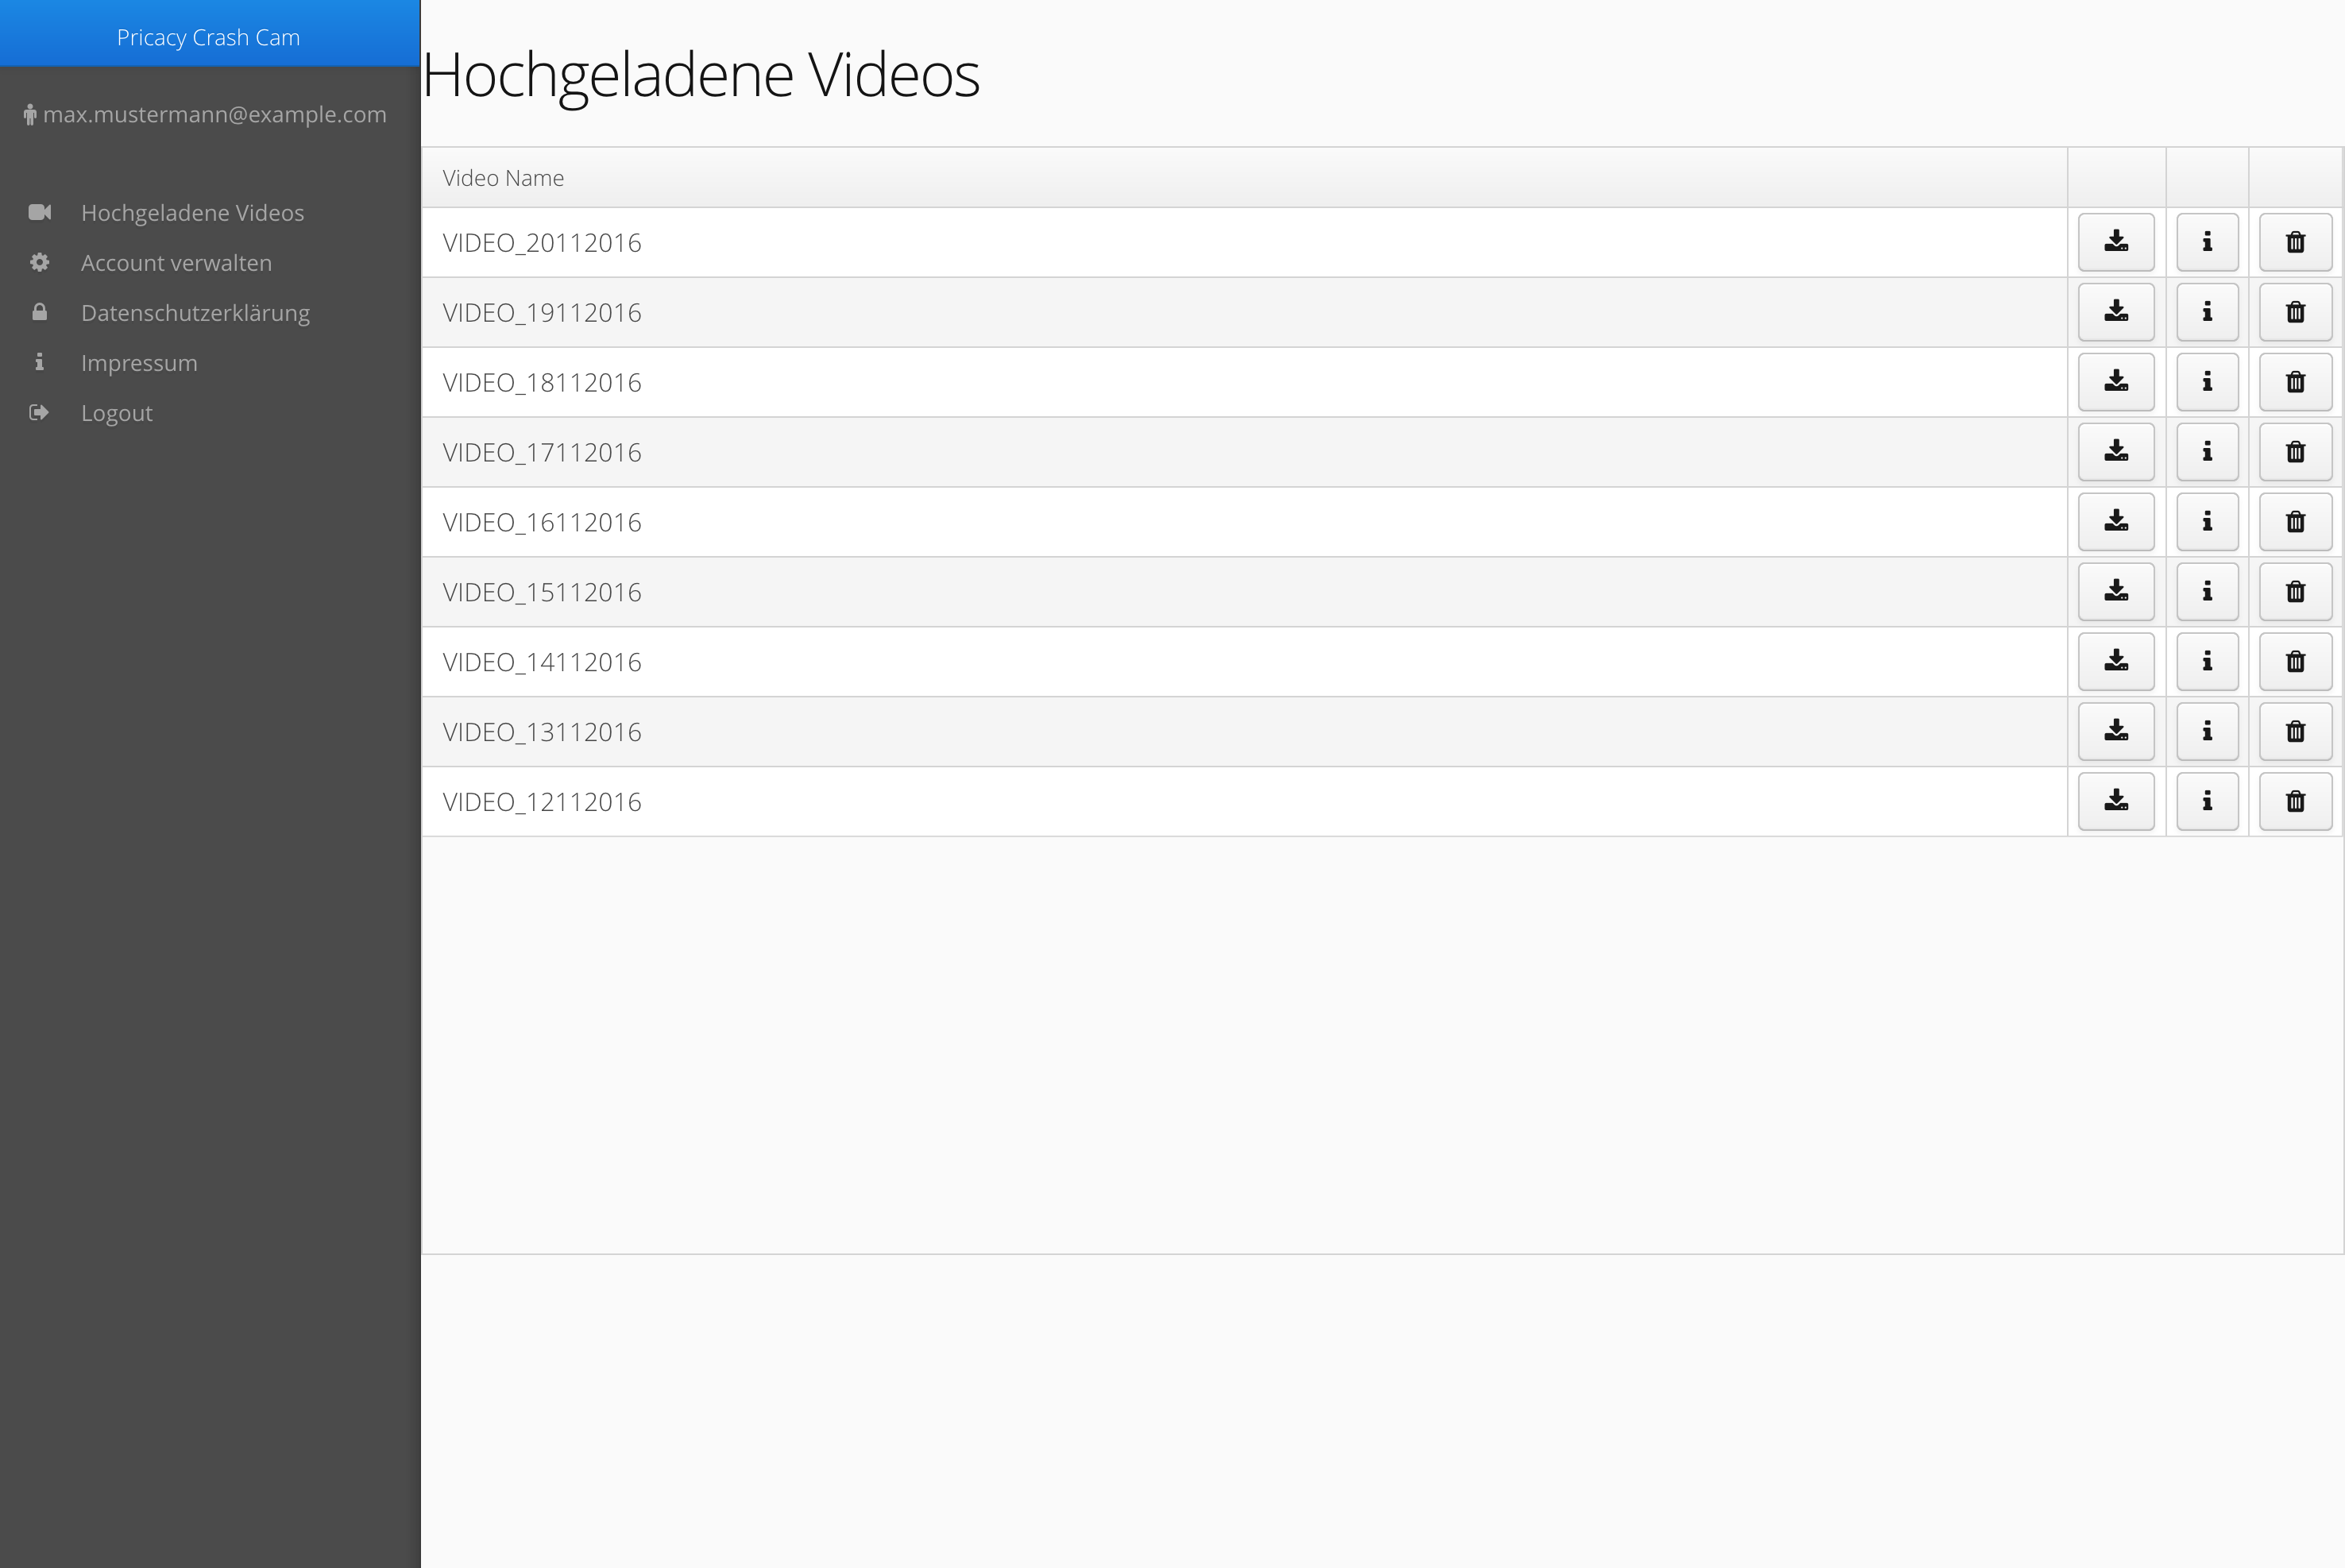
\includegraphics[width=1\textwidth]{subtopicsFuncspec/Res/UI-Demos/Webinterface.png}
\begin{figure}
	\centering
	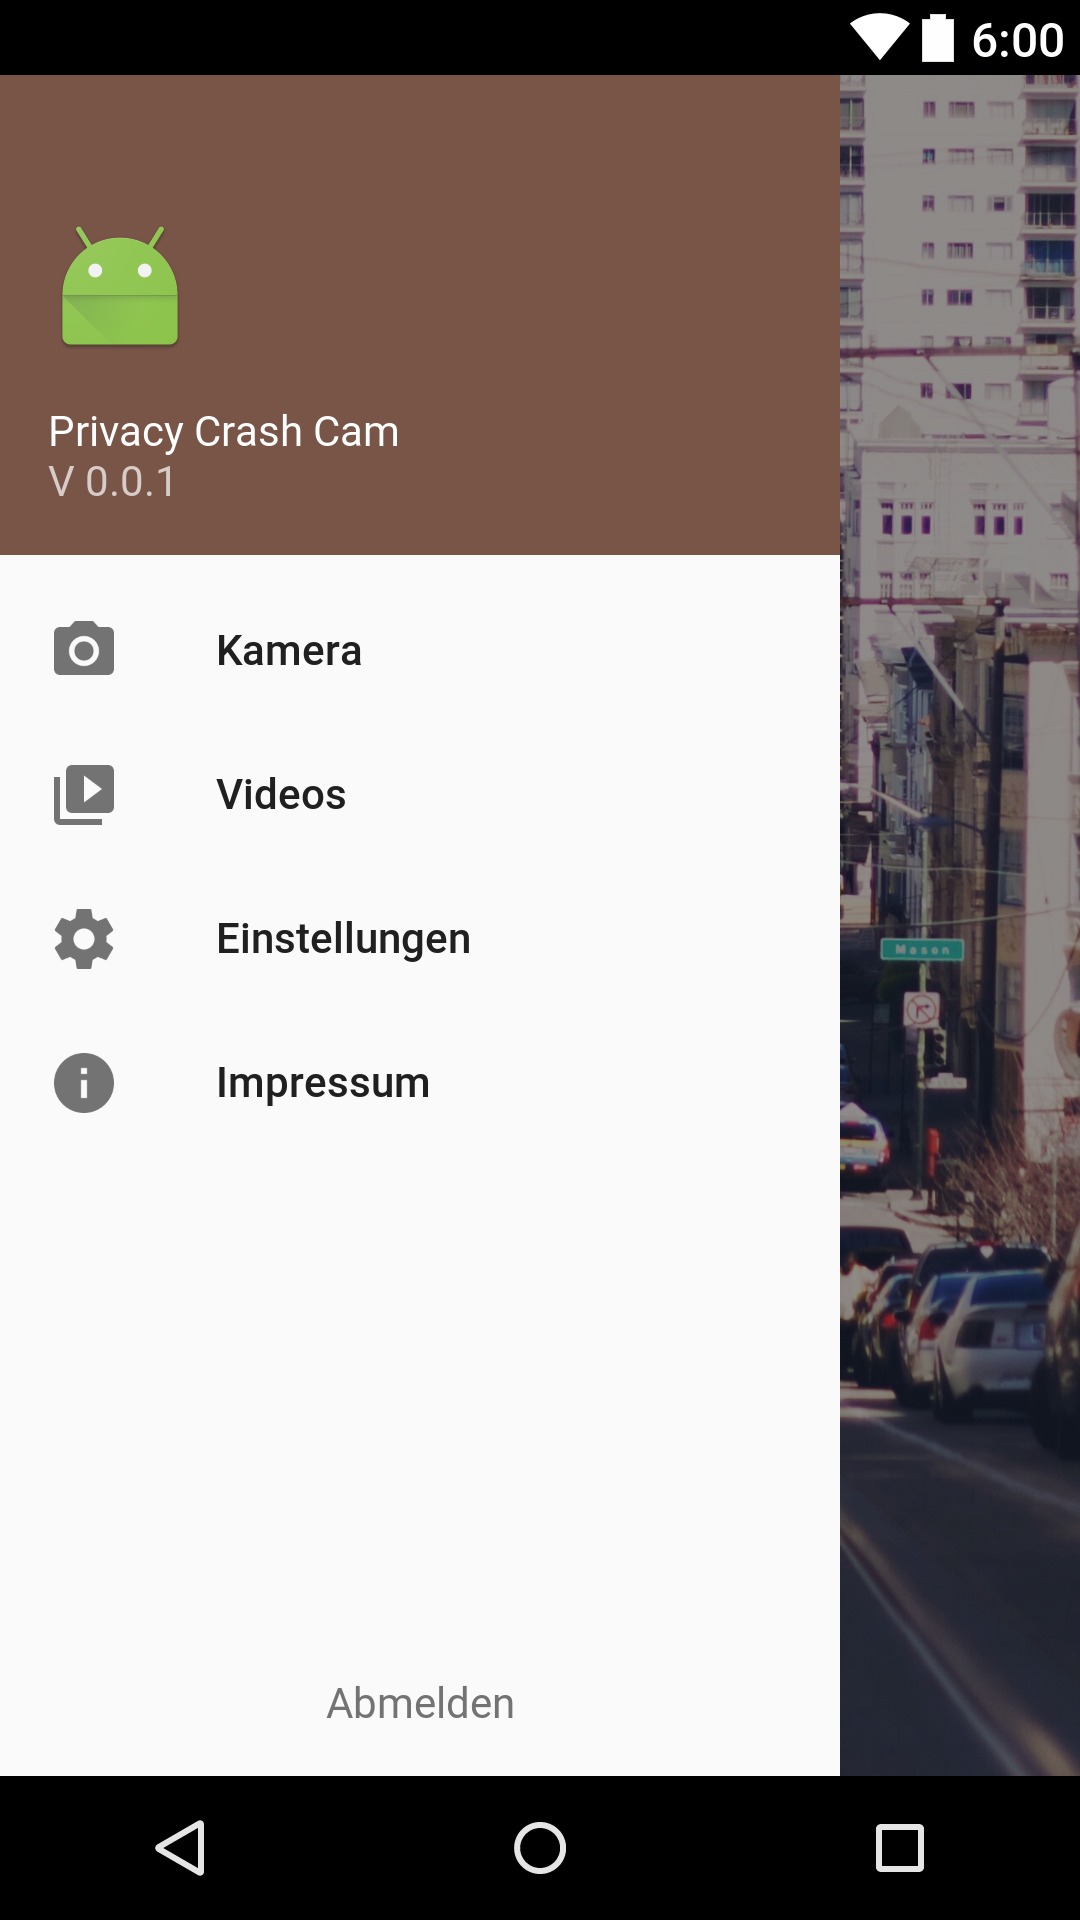
\includegraphics[width=0.33\textwidth]{subtopicsFuncspec/Res/Mockups/Portrait_camera_view_menu.png}
	\caption{Menü}
\end{figure}
\begin{figure}
	\centering
	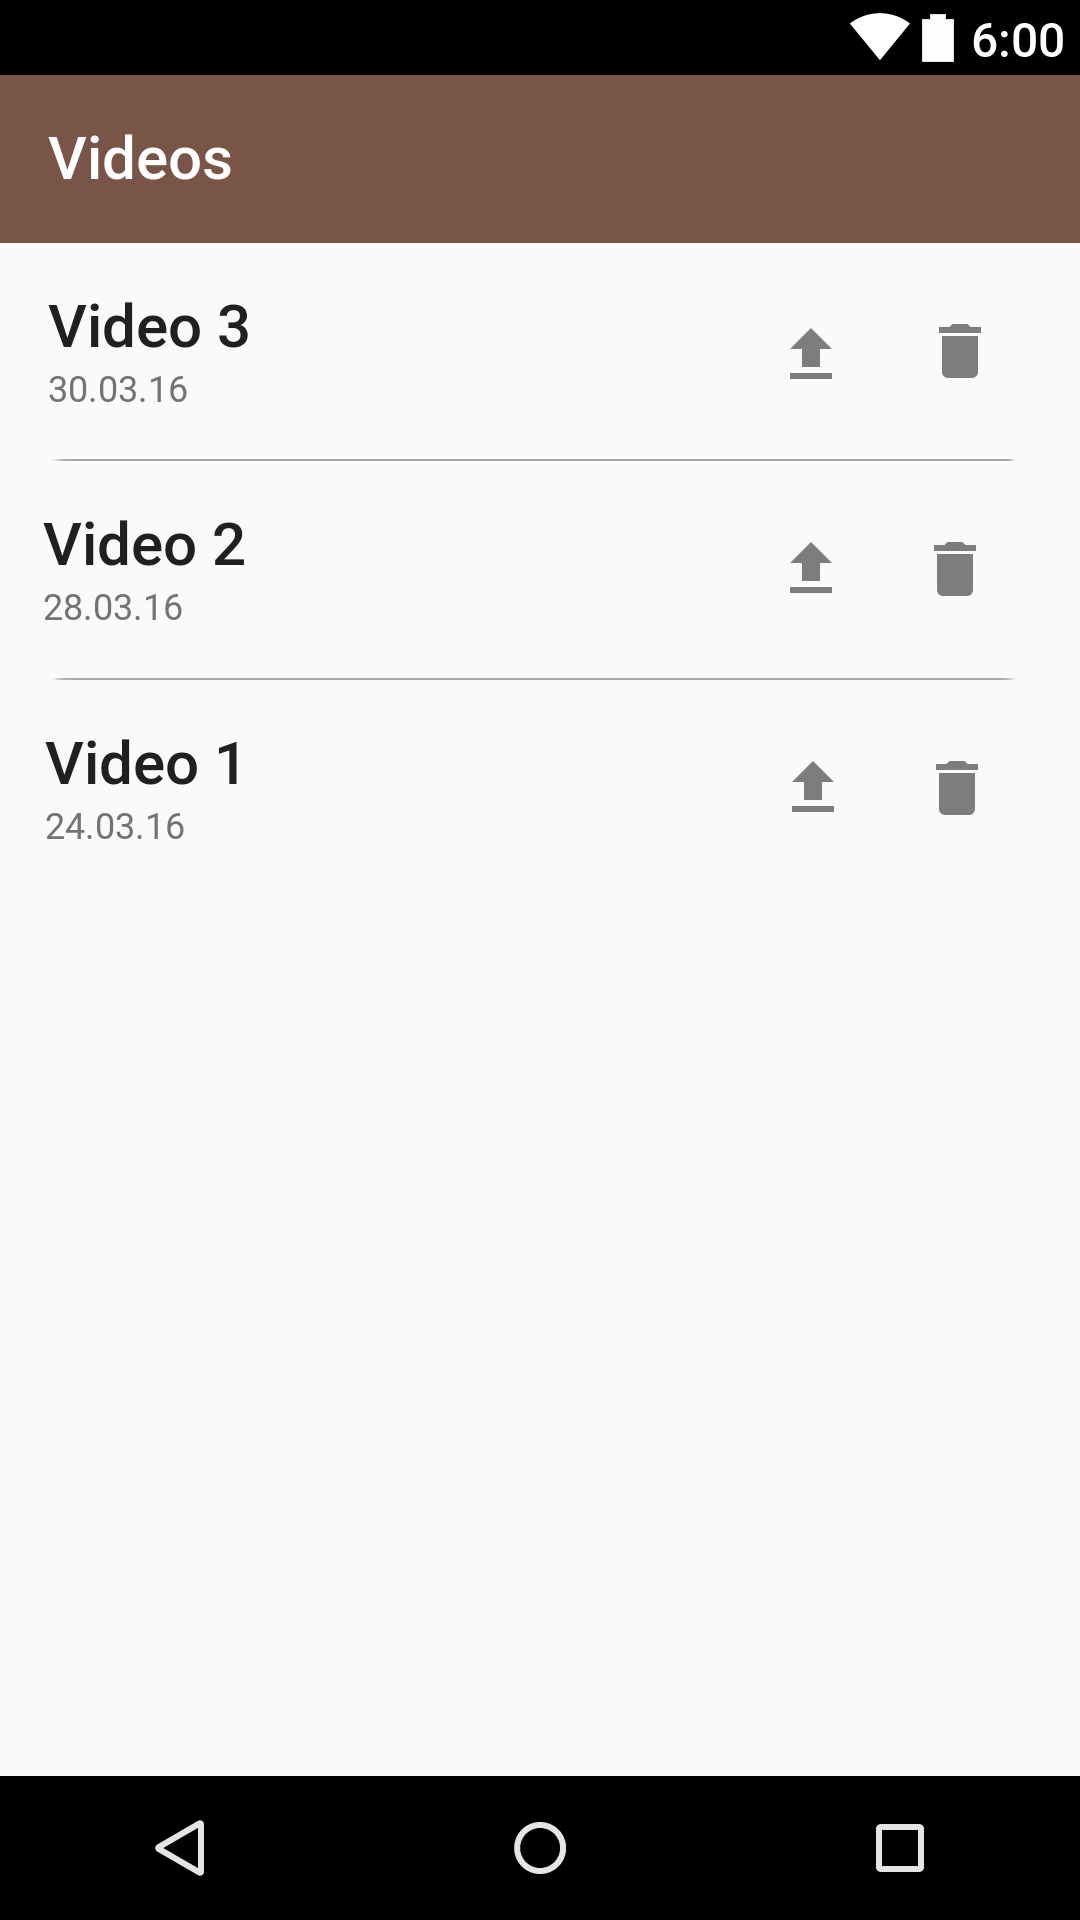
\includegraphics[width=0.33\textwidth]{subtopicsFuncspec/Res/Mockups/Videos_list1.png}
	\caption{Videos}
\end{figure}
\begin{figure}
	\centering
	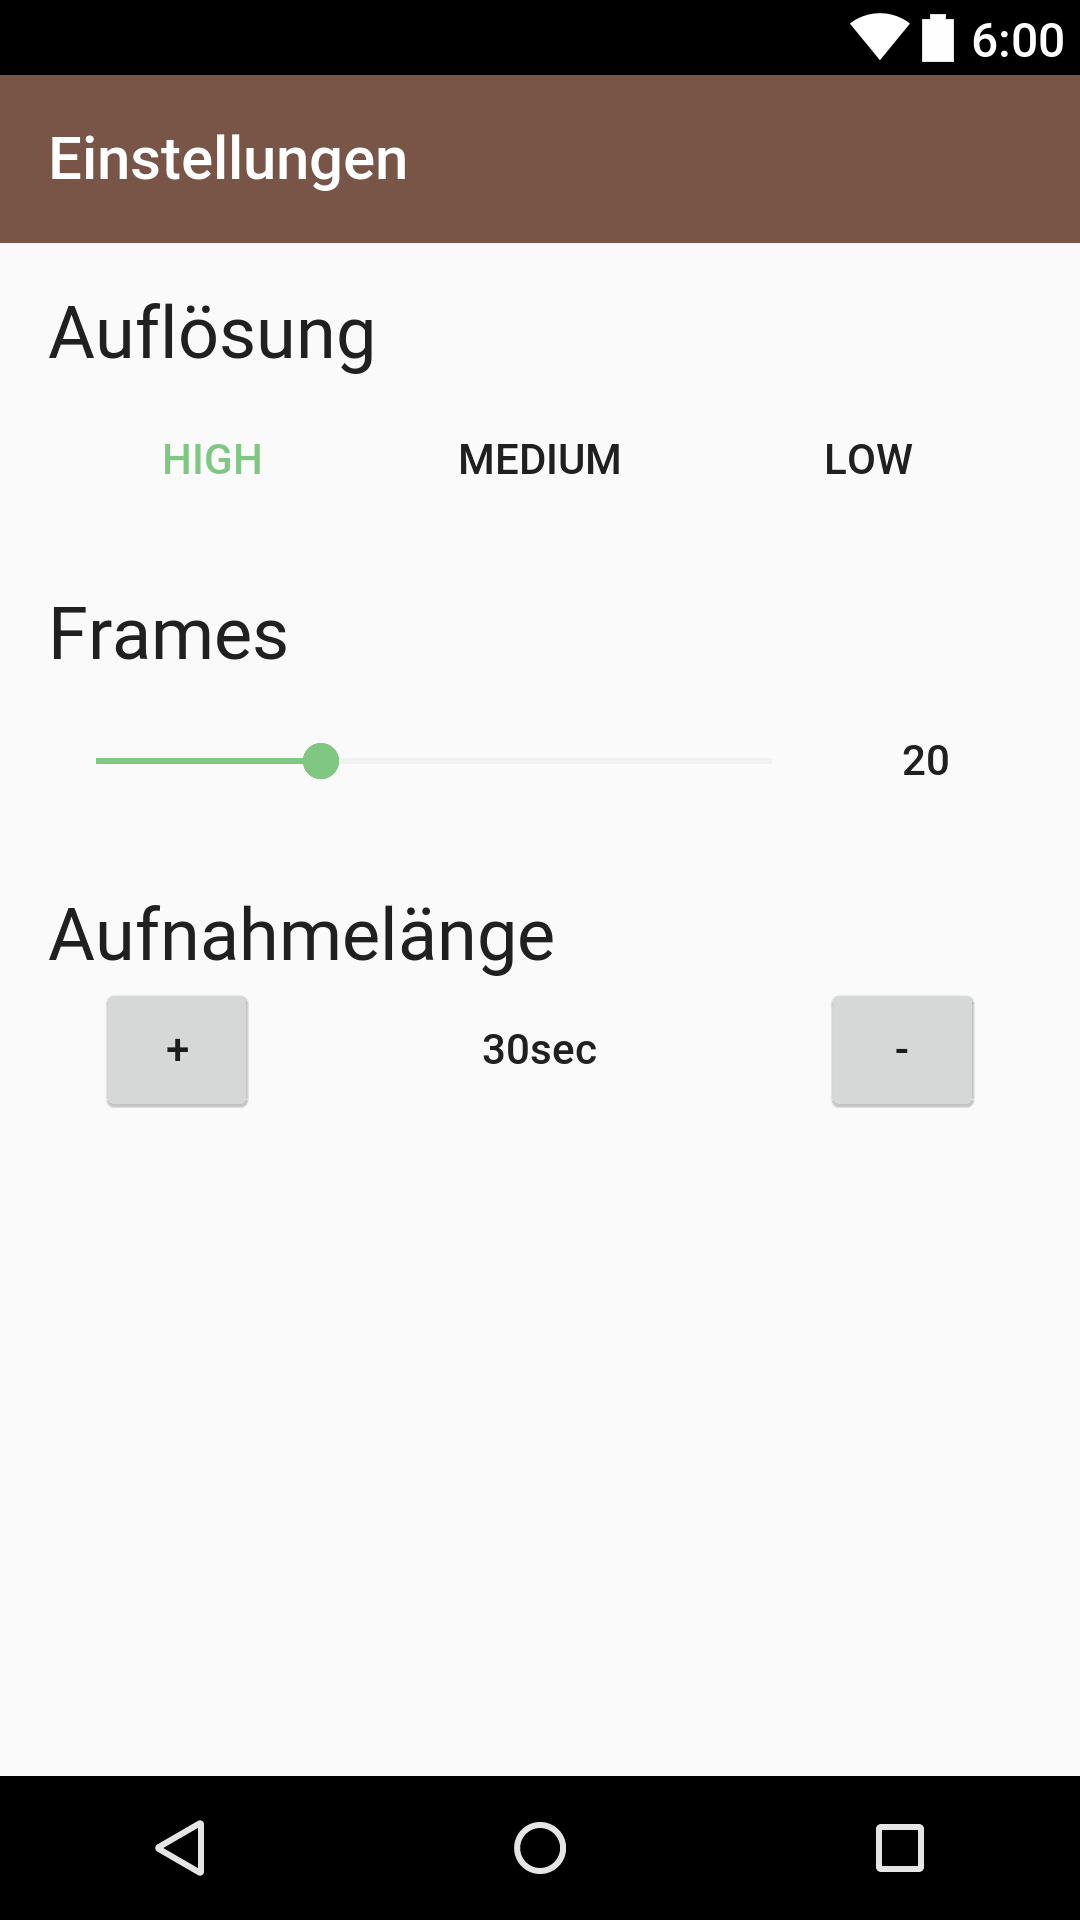
\includegraphics[width=0.33\textwidth]{subtopicsFuncspec/Res/Mockups/Settings1.png}
 	 \caption{Einstellungen}
\end{figure}

\newpage

\section{Verschlüsselung} \label{sec:Verschlüsselung}

Um den Datenschutz zu gewährleisten, ist die Verschl\"usselung eine zentrale Funktion der App und des Web-Dienst. Hierbei m\"ussen die Videos vor der Anonymisierung verschlüsselt gespeichert werden. Dabei wendet die App beim Persistieren eine hybride Verschlüsselung an. Die hybdride Verschlüsselung verbindet dabei die Geschwindigkeit von symmetrischer Verschlüsselung mit der Sicherheit asymetrsicher Verschlüsselung.\\
Zunächst wählt die App einen zufälligen symmetrischen Schlüssel. Mit diesem Schlüssel wird das Video symmetrisch verschlüsselt. Anschließend wird der Schlüssel asymmetrisch mit dem öffentlichen Schlüssel des Web-Dienst verschlüsselt. \\
Als kryptographisches Verfahren werden hierbei AES für die symmetrische und RSA für die asymetrische Verschlüsselung verwendet.


\newpage
\printglossaries
\newglossaryentry{Android}
{
  name = Android,
  description = {Android ist ein von Open Handset Alliance entwickletes Betriebssystem, sowie eine Software Platform für mobile Geräte(\gls{Smartphone} und \gls{Tablet}). Dabei handelt es sich um eine freie und quelloffene Software, die auf einem Linux-Kernel basiert},
}
\newglossaryentry{App}
{
  name = App,
  plural = Apps,
  description = {Als Applikationen, oder eher als Kurzform App bekannt, wird eine Anwendungssoftware auf einem Betriebssystem bezeichnet. Bei mobilen Applikationen wird zwischen verschiedenen Typen unterschieden. Zum einen existieren native Apps (Platformabhängig), Web-, und Cross-Plattform-Apps (Platformunabhängig)},
}
\newglossaryentry{IDE}
{
	name = IDE,
	plural = IDEs,
	description = {Eine IDE (integrierte Entwicklungsumgebung) ist eine Sammlung von Programmen zur Softwareentwicklung},
}
\newglossaryentry{API}
{
  name = API,
  description = {Eine API (Application Programming Interface), auf deutsch Programmierschnittstelle genannt, macht es einfacher ein Programm zu entwickeln, indem sie vorgefertigte Funktionen zur Verfügung stellt. Diese werden mit einem Softwaresystem mitgeliefert und stellen eine Programmieranbindung auf Quelltext-Ebene dar},
}
\newglossaryentry{Web-Dienst}
{
  name = Web-Dienst,
  plural = Web-Dienste,
  description = {Web-Dienste (auch Web-Service) sind Softwareanwendungen, die über ein Netzwerk bereitgestellt werden},
}
\newglossaryentry{Web-Interface}
{
  name = Web-Interface,
  plural = Web-Interfaces,
  description = {Ein Web-Interface (auch Web-Schnittstelle), bezeichnet eine Schnittstelle zu einem System, die über ein Netzwerk angesprochen wird. Dabei wird unterschieden zwischen einer grafischen Benutzerobfläche und einem \gls{Web-Dienst}, durch das mit einem anderen System interagiert werden kann},
}
\newglossaryentry{G-Sensor}
{
  name = G-Sensor,
  plural = G-Sensoren,
  description = {Der G-Sensor (bekannt als Beschleunigungssensor), ist ein Sensor der die Beschleunigung in verschiedene Bewegungsrichtungen misst},
}
\newglossaryentry{Metadaten}
{
  name = Metadaten,
  description = {Metadaten enthalten Informationen über andere Dateien. Diese Informationen werden bei der Ansammlung größerer Datenmengen (wie Dokumente, Datenbanken oder Dateien) benötigt, um diese zu verwalten},
}
\newglossaryentry{persistieren}
{
  name = persistieren,
  description = {Die Persistierung (Verb: persistieren) wird in der Informatik häufig als ``nicht flüchtige Datenspeicherung'' definert. Dadurch wird die Funktion, Daten oder Objekte über längere Zeit zu speichern, beschrieben},
}
\newglossaryentry{anonymisieren}
{
  name = anonymisieren,
  description = {Mit Anonymisierung bezeichnet man den Vorgang, personenbezogene Daten so zu ändern, dass diese Daten nicht mehr einer Person zugeordnet werden können},
}
\newglossaryentry{E-Mail}
{
  name = E-Mail,
  plural = E-Mails,
  description = {Ein E-Mail ist eine briefähnliche Nachricht, die zwischen Personen mit bestimmten Netzwerkverbindungen auf einem definierten System verschickt werden kann},
}
\newglossaryentry{Smartphone}
{
  name = Smartphone,
  plural = Smartphones,
  description = {Ein Smartphone ist ein Mobilfunkgerät, das die Funktionalität eines herkömmlichen Mobiltelefons überschreitet und diese mit umfangreicheren Computer-Funktionalitäten erweitert},
}
\newglossaryentry{Push-Benarichtigung}
{
  name = Push-Benarichtigung,
  plural = Push-Benarichtigungen,
  description = {Push-Benachrichtigungen sind Meldungen, die ohne das Öffnen der jeweiligen \gls{App} auf dem \gls{Smartphone} erscheinen},
}
\newglossaryentry{Livestream}
{
  name = Livestream,
  plural = Livestreams,
  description = {Ein Livestream (auf deutsch Echtzeitübertragung), ist das Öffnen eines digitale Übertragungskanals. Über diesen kann ein Datenstrom, bestehend aus Video- und Audiomaterial in Echtzeit verschickt und empfangen werden},
}
\newglossaryentry{Tablet}
{
  name = Tablet,
  plural = Tablets,
  description = {Tablets (auch bekannt als Tablet-PC), sind flache, tragbare Computer. Sie besitzen meist die gleichen Standartfunktionen wie ein normaler PC (möglicher Anschluss von Maus und Tastatur, WLAN), aber auch Funktionen eines \gls{Smartphone} (Multitouchscreen oder Bedienung per Stift)},
}
\newglossaryentry{iOS}
{
  name = iOS,
  description = {iOS ist ein von Apple entwickelte mobiles Betriebssystem für deren hergestellte Mobilgeräte, wie das iPhone},
}
\newglossaryentry{Windows Phone}
{
  name = Windows Phone,
  description = {Windows Phone ist ein Betriebssystem für Smartphones, das von Microsoft entwickelt wurde},
}
\newglossaryentry{Ringpuffer}
{
  name = Ringpuffer,
  description = {Der Ringpuffer (oder auch in der Informatik als Warteschlange bekannt) ist eine Datenstruktur, bei der diejenigen Elemente, die zuerst gespeichert wurden, auch zuerst wieder aus dem Speicher entnommen werden, wenn dieser vollläuft},
}
\newglossaryentry{RSA}
{
  name = RSA,
  description = {RSA ist ein populäres asymmetrisches kryptographisches Verfahren, das auf dem Faktorisierungsproblem beruht},
}
\newglossaryentry{Kryptografisches Verfahren}
{
  name = Kryptografisches Verfahren,
  description = {Unter Kryptografie versteht man die Lehre von Geheimschriften. Kryptographische Verfahren werden dazu verwendet Dateien zu Verschlüsseln und diese somit vor nicht autorisierten Lesern zu schützen},
}
\newglossaryentry{Responsive-Design}
{
  name = Responsive-Design,
  description = {Responsive Webdesign bezeichnet die Gestaltung von Oberflächen in der Form, dass diese sich an die Eigenschaften des Endgeräts anpassen},
}
\newglossaryentry{AES}
{
  name = AES,
  description = {AES (Advanced Encryption Standard), ist ein standardisiertes symmetrisches Verschlüsselungsverfahren, das auf Blockverschlüsselung beruht},
}
\newglossaryentry{Java-Servlet}
{
  name = Java-Servlet,
  plural = Java-Servlets,
  description = {Als Java-Servlets bezeichnet man Klassen in Java, die Fähigkeiten eines Webservers erweitern, indem sie Anfragen von Clients beantworten und entgegennehmen. Dabei ist die Besonderheit die dynamische Antworterstellung, die je nach Anfrage variiert},
}
\newglossaryentry{Hash-Code}
{
  name = Hash-Code,
  description = {Hashing ist eine Funktion, die aus einem Klartext beliebiger Länge eine Zeichenkette fester Länge, den Hash-Code, erstellt. Dabei ist es nicht direkt möglich aus dem Hash-Code auf die ursprüngliche Zeichenkette zu schließen},
}


%end content

\end{document}

